
%%% Chapter 4: A Reinforcement Learning Approach for Performance-aware Reduction
%%%            in Power Consumption of Data Center Compute Nodes
%%% Based on: IC2E 2024 paper
%%% Authors: Akhilesh Raj (Vanderbilt University), Swann Perarnau (Argonne National Laboratory),
%%%          Aniruddha Gokhale (Vanderbilt University)

\chapter{A Reinforcement Learning Approach for Performance-Aware Reduction in Power Consumption of Data Center Compute Nodes} \label{CH4_IC2E}

% Set the figure path for this chapter
\graphicspath{{Papers/IC2E/}}

\section*{Abstract}
As Exascale computing becomes a reality, the energy needs of compute nodes in cloud
data centers will continue to grow. A common approach to reducing this energy demand
is to limit the power consumption of hardware components when workloads are
experiencing bottlenecks elsewhere in the system. However, designing a resource
controller capable of detecting and limiting power consumption on-the-fly is a
complex issue and can also adversely impact application performance. In this chapter,
we explore the use of Reinforcement Learning (RL) to design a power capping policy
on cloud compute nodes using observations on current power consumption and
instantaneous application performance (heartbeats). By leveraging the Argo Node
Resource Management (NRM) software stack in conjunction with the Intel Running
Average Power Limit (RAPL) hardware control mechanism, we design an agent to
control the maximum supplied power to processors without compromising on application
performance. Employing a Proximal Policy Optimization (PPO) agent to learn an
optimal policy on a mathematical model of the compute nodes, we demonstrate and
evaluate using the STREAM benchmark how a trained agent running on actual hardware
can take actions by balancing power consumption and application performance.

\section{Introduction} \label{ch3:sec:Introduction}
Cloud data centers are increasingly providing a variety of high performance computing nodes 
including hardware accelerators to support the needs of a range of compute-intensive 
applications including various machine learning training/inferencing and scientific
applications. In these setups, a large number of compute nodes are networked together via
high-speed networks to provide high performance computing capabilities. 
%Production-quality high-performance computing (HPC) systems refer to that class of machines where a large number (in the range of hundreds or thousands) of compute-intensive servers are networked together using a high-speed network.
% Such an HPC machine consists basically of three main components - 1) compute nodes 2) network and 3) storage. These three components are interconnected across high speed networks to form a typical HPC cluster as shown in Fig.~\ref{fig:HPC}. Each compute node works independently and in parallel toward completing a common task and has access to its own individual or shared resources. The input or the supplied power, being one among them, is the source of energy-on-demand for a node and also provides the users with a leverage to regulate its performance~\cite{mantovani2018performance}. In this paper, we attempt to design an RL based framework to regulate the supplied power to an HPC node provided the performance to power ratio will be maximized.
% Akhilesh, without stating the problem, it makes no sense to say what this paper does. SO I am commenting here and moving elsewhere. 
% Moreover, the para is extremely long so breaking them in appropriate places
%In this paper, we attempt to design a method to reduce the consumed power without effecting the execution time of a workload.
% \begin{figure}[htb]
%     \centering
%     \vspace{-0.5cm}
%     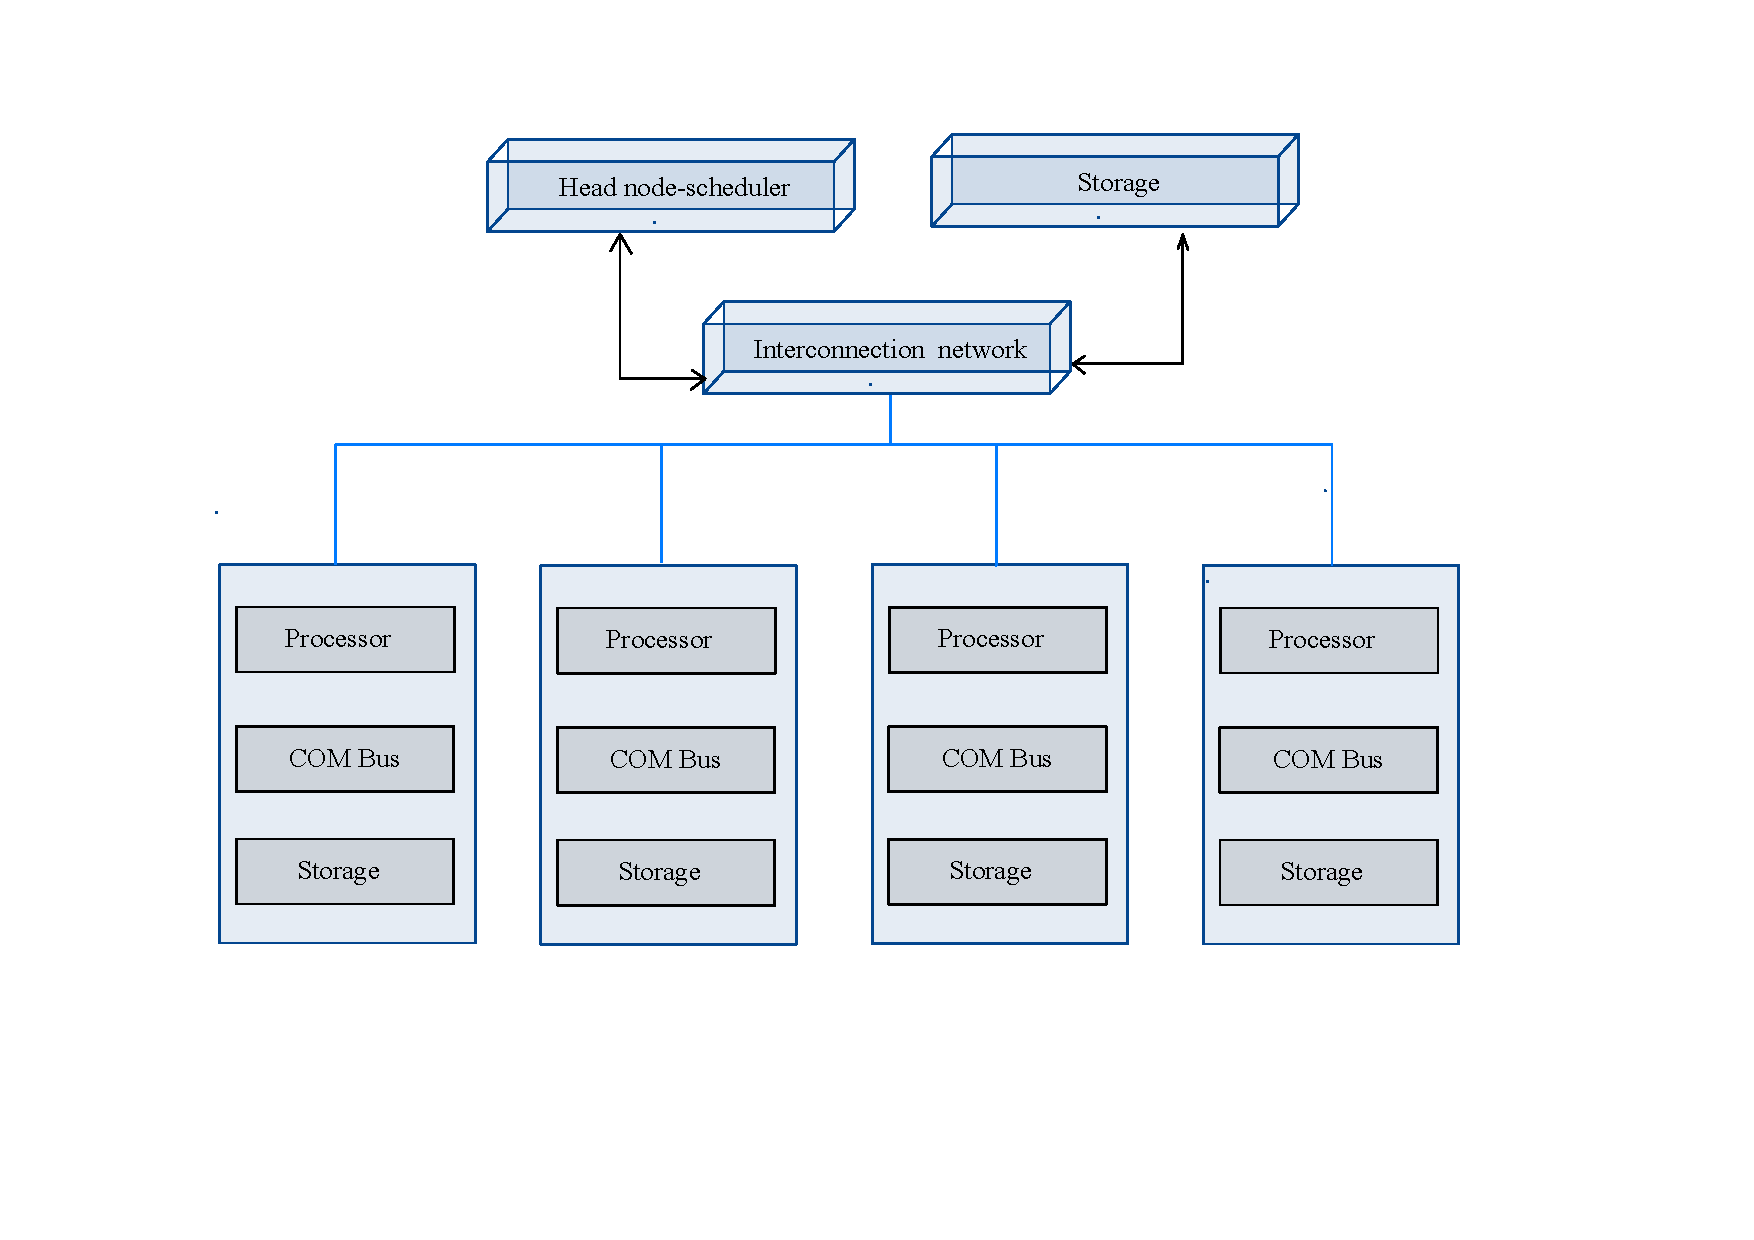
\includegraphics[trim={3cm 1cm 4cm 1cm},clip,width=\linewidth]{Figures/HPC.pdf}
%     \vspace{-2cm}
%     \caption{An HPC cluster architecture}
%     \label{fig:HPC}
%     \vspace{-0.5cm}
% \end{figure}
This growth, however, has given rise to several challenges, notably in the areas of energy efficiency.  
For instance, Darrow et al. in ~\cite{darrow2009opportunities} pointed out that data centers consume 10-50 times the energy per floor space compared to any other commercial building and the consumed energy constitute 2\% of the total US energy consumption.
Multiple surveys and studies~\cite{darrow2009opportunities,koomey2011growth,koot2021usage,shalf2020future,dayarathna2015data} have shown that the global power consumption for computing is expected to increase in the upcoming years. 

Consequently, research on data center power consumption has gained considerable attention since the publication of initial statistics on its energy usage, which illuminated the rapidly increasing demands of servers worldwide~\cite{koomey2011growth}.
% The data center power consumption has been a hot topic of research ever since some of the initial statistics on its power consumption ~\cite{koomey2011growth} shed light on the growing demands of its servers across the world.
A more recent survey shows that the growing demands of these data centers are not in proportion with their efficiency despite the technological innovations ~\cite{koot2021usage}. In other words, the rate at which the power consumption increases across the generations of data centers are higher than the rate of growth in their efficiency. 
\iffalse
% Might be too repetitive
The global data center power is expected to rise from 1.16\% to 1.86\% by the end of this decade, making it one of the most expensive infrastructure to maintain. 
\fi 
Within the data center, almost 86\% of the total power consumption is equally shared between the cooling system and servers~\cite{shehabi2016united}, which makes the power consumption of compute nodes an important issue that needs to be addressed. 
\iffalse
% Need to move this sentence later
In this paper, we solely focus on the power consumption by the compute nodes, while the study on HVAC consumption remains a scope for future works.
\fi 

% Methods to reduce the server node power consumption can be broadly classified into minimization of power dissipation and minimization of power supply based approaches. 
In the context of reducing compute node power consumption, various methods have been proposed that can be broadly classified into two categories: those that focus on minimizing power dissipation and those that focus on minimizing power supply. These approaches aim to reduce the overall energy consumption of compute nodes, while maintaining their performance and functionality.
The former is strictly a Very Large Scale Integration (VLSI) design problem, while the latter is a cyber-physical systems problem, which can be dealt with using efficient power management algorithms (i.e., control system design), which is the focus of this paper. 
% \todo{conflicting sentences: without affecting the execution time, or not let vary significantly, not both. Also, technically we end up with the same goal as in europar: bounding execution time degradation}

Specifically, we design a method to reduce the consumed power without any noticeable impact on the execution time of a workload. Through our work, we achieve regulation of the average supplied power using a reinforcement learning (RL) agent, trained using a mathematical model which relates the progress made by the application towards the completion of its scientific-goal to the power cap (pcap) of RAPL actuators. Additionally, the goal is to not let the execution time vary significantly when compared to that with maximum power execution.
% so that the execution time of a standard benchmark application remain the same as compared to the maximum power execution.


To that end, we present a real-time, dynamic power management scheme that is based on observing both time-aware and power-aware variables as a solution to the power management problem of the high performance compute nodes. 
% We will be detailing more about the evolution of this work in the next section \ref{sec:Related_work}.
% This paper describes in detail the steps for using an RL agent to control the PCAP for an HPC node that uses RAPL actuators and sensors while keeping the performance at maximum. 
In our work, the RL agent observes the progress made by the application towards completing its scientifc goal at each instant and makes a decision on the power requirement for the next time step based on this observation. The action, which is based on this decision, is taken by setting the running average power limit (RAPL) power caps at the computed value. RAPL is an interface available on modern Intel processors to monitor and control the energy consumption of various power domains. Our approach is incorporated in the Argo Node Resource Management (NRM) stack~\cite{anrm}.
%The evolution of this work is detailed in the next Section \ref{sec:Related_work}.

% In our work, the observation made by the agent consists of the feedback from a time-based application execution (application heartbeats) which also depends on the PCAP given in the previous instance. On observing this parameter, our objective is to analyze the requirements of a processor running a standard benchmark application and suggest a suitable PCAP required for the next iteration.  
% {The contributions of this paper are:
% \begin{itemize}
% \item A novel RL based algorithm that relies on the system model for training,
% \item A software stack that automates the training process once the observation space is decided,
% \item An easy to implement hardware based algorithm with open source repository with code for researchers to test and extend the results.
% \end{itemize}} The results presented in Section~\ref{Sec:Results} show how an RL-agent can effectively limit the power consumption in an HPC node while minimizing the execution time of a benchmark workload. 

The key contributions of this paper are the following:
\begin{itemize}
\item A novel RL-based algorithm that relies on the system model for training.
\item An RL-based architecture employing the trained model to control the compute node within a desired operational region, while utilizing real-time progress measurements.
\item An implementation of the algorithm with an open-source repository for researchers to test and extend the results.
\end{itemize}
 % The results presented in Section V-A show how an RL-agent can effectively limit the power consumption in an HPC node while minimizing the execution time of a benchmark workload
% \todo{I don't like this distinction between hardware based and software based. The controller is in software, we're just using a hardware actuator to apply it.}

The remainder of this paper is structured as follows: In Section ~\ref{sec:Related_work}, we review existing algorithms in power and performance optimization. Section~\ref{ch3:sec:Background} presents the necessary background for this paper, including the RL algorithm, hardware and software stacks, and packages used in the experiments. Section ~\ref{ch3:sec:Methodology} outlines the proposed algorithm and workflow in the context of compute nodes. In Section ~\ref{sec:Eval}, we present the experimental design and implementation, along with the results and analysis. Finally, Section ~\ref{ch3:sec:Conclusion} provides conclusions including a brief summary, the impact of this work and future opportunities. 
%We acknowledge the supporting hardware and software stack providers in Section \ref{sec:Acknowledgments} .


% The rest of the paper is organized as follows: Section~\ref{sec:Related_work} provides insights into a sampling of existing algorithms in power and performance optimization. Section~\ref{ch3:sec:Background} provides the required background to make this paper self-contained, with a focus on the RL algorithm, hardware and software stacks, and packages used for the experiments. Section~\ref{ch3:sec:Methodology} presents the proposed algorithm and workflow of the method in light of the HPC nodes. Section~\ref{sec:Design} presents the design and implementation of the experiment, the obtained results and its analysis. Section~\ref{ch3:sec:Conclusion}, provides the conclusions of the paper with a brief summary and impact of this work for future opportunities, before acknowledging the supporting hardware and software stack providers, in section \ref{sec:Acknowledgments} 

\section{Related Work}\label{sec:Related_work}

% There is a growing demand for the research on machine learning methods for performance and power optimization in compute nodes ~\cite{chen2015distributed}. 
% The research can be broadly classified into two categories based on the algorithms used for power control: software and hardware approaches. 
{Prior methods for regulating the performance on HPC nodes can be classified either as a Power-aware scheme~\cite{hsu2005power,patki2015practical} or as a Time-aware scheme~\cite{sadrosadati2019itap,qiu2012three}. A power-aware scheme is designed with the primary objective of minimizing power consumption while still achieving acceptable performance levels. The main focus of this scheme is to optimize energy usage and reduce power consumption in computing systems. Power-aware schemes may employ techniques such as dynamic voltage and frequency scaling (DVFS), power capping, power gating, and other power management methods to control and regulate power usage based on workload and system conditions. The goal is to maximize energy efficiency and reduce the overall carbon footprint of the computing system. Time-Aware Scheme on the other hand, prioritizes meeting specific time or performance requirements, often associated with critical real-time or time-sensitive applications. The main objective of a time-aware scheme is to ensure that tasks or processes are completed within predefined time constraints or deadlines. In time-aware schemes, performance and response time take precedence over power efficiency. These schemes may use techniques like aggressive clock frequency scaling, parallelism, or task prioritization to meet the time requirements of critical applications.} This section provides an overview of some of these methods which also explains why there is a growing demand for machine learning based methods for the power and performance control that has lead to the proposed work. 
% We will also address why there is a growing demand for the researches on machine learning based methods for power and performance control.

Our prior work~\cite{caglar2014iplace} researched software approaches for power optimization using duty cycle, voltage and frequency scaling, wherein we used machine learning techniques to model the application performance and hardware characteristics, and use these models to guide the placement decisions.
% \todo{not relevant from here} \cite{felter2005performance} presents a detailed performance analysis of amazon EC2 with reference to its constrained memory and network resources. The software approach used in the EC2 for application management, shows room for improvement accounting to the fact that the targeted scalability was not obtained and was not a cost effective alternative. \cite{cochran2011pack} discussed an effective way of packing workloads minimizing the amount of user interventions required when moving an application across systems. This system was shown effective while running complex applications that require specific libraries, configurations and dependencies and therefore was not generalizable.  Software approaches always have the problem of delayed convergence and slowness.
% % Using learning based schemes, to maximize performance under given power caps, is another example of the software based methods.
% \cite{sayadi2017machine} studied the performance of state-of-the-art machine learning methods for feature extraction of a given work load, to determine the composite core architecture configurations, for determining the design of a heterogeneous system architecture.\todo{until here} 
But, the choice of method highly depended on the hardware under consideration.
Similarly, Jung et al. \cite{jung2010supervised} proposes a supervised learning based power management for multi-core processors. However, such algorithms are not always reliable due to the need for training data prior to the implementation of software-based optimization. 
% \todo{avoid past tense when talking about current tech}

On the other hand, methods that deal with system architecture that set the input power based on the system requirements converges faster. For example, a RAPL-based scheme supports a variety of algorithms that relies on hardware-based control for power capping on Intel processors~\cite{david2010rapl}. But the automation/feedback required for the processor to determine the power requirements based on the application it runs is not detailed in the paper.
Similarly Raghavendra et al. ~\cite{raghavendra2008no} utilizes a controller to stop the supplied power that is being delivered to the subsystems, by detecting the no-load zones in the application during its execution. Utilizing the technique, they are able to regulate the power to finer granularities. But, the efficiency of detecting the workload characteristics is not at the best, since the research focuses only on the hardware centric approach which is the main contribution of the paper.

Zhang et al. ~\cite{zhang2016maximizing} later came up with a hybrid method, combining software and hardware based methods to control the power supply, which showed significant improvement over the other methods. The authors combined the efficiency of the software-based approaches like DVFS, Task Scheduling etc. and the timeliness of the hardware approaches like Power Gating, Voltage regulators etc. together by reducing the time it takes to implement a power cap on the RAPL sensor from the moment its value is set. But a workload-based adaptive control of power was not considered here. Petoumenos et al. ~\cite{petoumenos2015power}, through their research give a comparative analysis of the software, hardware and hybrid approaches towards the power optimization in compute nodes.

Cerf et al. in her recent research  ~\cite{cerf2021sustaining} proposed a control theoretical approach to understand the possible operating regions of a compute node at which the performance decay is minimized under a reduced power supply. A classical proportional-integral-derivative (PID) controller was designed to impose power cap (PCAP) for RAPL actuators on an Intel(R) Xeon(R) Gold 6126 CPU by using performance feedback from the compute nodes~\cite{ramesh2019understanding}.
% \todo{heartbeats are from instrumented applications}. 
The RAPL actuators comprising a control knob or the PCAP knob and a time-window knob were used to regulate the average power given between two sampling intervals to a compute node. A mathematical model formulated using static characterization was used for the design of the controller. The controller was shown to be working for the compute nodes by making it track a user-computed set-point for the desired performance. While an adaptive controller~\cite{hawila:hal-03765849} addressed model inaccuracies, reliance on a user-defined set point calls for an automated approach.
% particularly for time-varying workloads\todo{not a good idea to introduce a concept we don't actually use, evaluate, or solve, stream is not time-varying}. 
% Furthermore, the PID controller used was not optimal for the control problem addressed in this paper.
% Even though the model inaccuracies that showed up during the static characterization were later taken care of by using an adaptive controller~\cite{hawila:hal-03765849}, the dependency on a user-defined set point that could lead to incorrect response, called for an automated approach, especially when a time varying application workload is under consideration. Moreover, the PID controller used, is not a solution for the optimal control problem addressed in this paper.


\iffalse 
The methods of solving for optimal control problems generally relies on some of the standard concepts from optimal control theory, namely:
\begin{itemize}
\item Mathematically solving for a control law by solving the Hamilton-Jacobi-Bellman (HJB) equations, 
% using the mathematical model of the dynamic process,
\item Dynamic programming, and 
\item Reinforcement Learning. 
\end{itemize}
Where the first two methods rely exclusively on mathematical models, the RL based approach tries to learn a policy (a set of actions) by directly testing its utility on the application. The accuracy of the mathematical model is a big factor in determining the efficiency of model based RL methods ~\cite{ke2019learning}.
% In the real world applications, where external signals (disturbance, noise, attacks etc.) interfere and impart uncertainties to the system, a real time measurement of the participating signals are important for a better inference.
In real-world applications, external signals such as disturbances, noise, and attacks can introduce uncertainties to the system, making real-time measurement of participating signals crucial for accurate inference.
By using a mathematical model for designing a control, we generalize these uncertainties using a bounded signal and try to prove that the controlled signal is stable whereas in model-free approach the RL agent can observe these uncertainties using real-time measurements. Therefore the model-free approaches can deal with randomness than a fixed model approach. 
% But in this work we limit our approach to a model-based learning in-order to make full use of HPC node, towards executing the benchmark application.
% Also, in section \ref{Sec:Results} we will evaluate our method by comparing the execution time and the total energy consumed with that of a PI controller. In-order to assure similar environment for executing the standard benchmark workload, we need to take training of the RL agent outside of the HPC node, where the HPC node functioning will be realized using a mathematical model.
However, in this work, we focus on a model-based learning approach in order to fully utilize the capabilities of an HPC node for executing a benchmark application. In Section \ref{Sec:Results}, we evaluate our method by comparing its execution time and total energy consumption with that of a PI controller by them on the same HPC node. We will also evaluate the RL-based controller for the repeatability of results on the same hardware as well as on different hardware.
% To ensure a similar environment for executing the standard benchmark workload, we train the RL agent outside of the HPC node, where the functioning of the HPC node can be realized using a mathematical model
% \todo{poor phrasing, we use a model to simulation the HPC controlled environment}.

% RL being the most effective state-of-the-art tool for stochastic optimization with a guaranteed sub-optimal solution, is used in this work as an agent to compute the action values.
% But on the other hand, this paper, tries to explore the possibility of using RL for power optimization in HPC nodes, by relying on its mathematical model for training, thereby laying a foundation for the model-free approaches we will be dealing with in the future. By using a Proximal Policy Optimization (PPO) RL-agent, we were able to show that an optimal policy  could be learnt by using a mathematical model, that gave an optimal performance when tested on hardware.
% Akhilesh, "optimized" or "optimal" in the above? ALso, just because RL is sort of new and everyone is jumping on the bandwagon cannot be a justification alone for using the technique. We need some more stronger language justifying its choice in our solution.


Literature emphasis on two classes of state-of-the-art power management approaches based on the observation variables:
\begin{itemize}
\item Power-aware scheme ~\cite{hsu2005power,patki2015practical}, and
\item Time-aware schemes \cite{sadrosadati2019itap,qiu2012three}.
\end{itemize}
While the former measures and reallocates power based on observed usage of power, the latter measures the relative time between the communicating software and reallocates power based on timing differences. Some of the prior works like \cite{9139791,tsujita2022classifying} introduced a novel application-level power management, employing an in-situ analysis of application workflows that took into consideration both time and power feedback for its respective designs. 
\fi 

Considering the limitations in prior work, we emphasize the design of an optimal controller by solving the underlying power and performance optimization problem.  We propose a hybrid approach for determining the best operating power cap for a compute node by relying on the instantaneous performance analysis that is obtained using the state-of-the-art algorithms.

\section{Background}\label{ch3:sec:Background}
To make the paper self-contained, this section provides the necessary background on the concepts and technologies used.
%In this section we brief some of the imperatives to better understand the methodology in section \ref{ch3:sec:Methodology}. Beginning with the most important concept in the paper, the Reinforcement Learning, we expands on the basic software and hardware requirements used for the computational and experimental purposes. 
\subsection{Reinforcement Learning} \label{subsec:Reinforcement_Learning}
Reinforcement Learning (RL) iteratively improves a sequence of actions or strategy through continuous interactions with the environment over a finite or infinite amount of time traversed using discrete time steps. 
In this work we use an RL agent to learn an optimal control policy by constantly generating an action and evaluating it using a mathematical model that describes the relation between power cap  and progress made by the compute node while running an application. The RL problem can be mathematically formulated as a Markov Decision Process (MDP), where the agent interacts with an environment that is modeled as a set of states, actions, and rewards. 
% An MDP is defined as a tuple $(\mathcal{S}, \mathcal{A}, \mathcal{P},r,\gamma)$ representing the state space, a set of actions available to an agent, the unknown transition kernel, the reward function and the discount factor respectively. 
At each time step, the agent observes the current state, selects an action based on a policy, and receives a reward from the environment. The goal of the agent is to learn a policy that maximizes the expected cumulative reward over time. 
%RL algorithms can be divided into two main categories: model-based and model-free. Model-based algorithms learn a model of the environment, which is used to estimate the expected rewards of different actions. Model-free algorithms, on the other hand, directly estimate the value of different actions without explicitly modeling the environment. 
In this paper we use a model-based algorithm by employing a Proximal Policy Optimization (PPO)~\cite{schulman2017proximal} agent to learn the state transition and the reward functions, thereby learning the policy.

\iffalse
PPO is a model-free algorithm, meaning that it does not rely on a model of the environment. Instead, it updates the policy directly based on observed rewards and states. While PPO is not a model-based algorithm, it is possible to use a model-based approach in conjunction with PPO. For example, one could use a model-based algorithm to learn a transition function and reward function, and then use these models to generate simulated trajectories for the agent to learn from using PPO \cite{https://doi.org/10.48550/arxiv.1903.00374}. In this paper, the authors use a learned transition model in combination with PPO to train an agent for playing Atari games. The learned model is used to simulate trajectories for the agent, allowing for more efficient learning compared to directly interacting with the environment. This approach is known as model-based reinforcement learning with a learned model. 

A PPO \cite{schulman2017proximal} is a state of the art RL training algorithm that has demonstrated good performance on a variety of tasks, including control problems in robotics, games and other complex environments. It is relatively simple to implement and tune, while still providing strong performance. It is stable and efficient, allowing for faster convergence to optimal policies. Moreover, we will be relaxing this paper's dependency on the mathematical model in our future work, where we will be using the model-free learning capability of the PPO agent for training it on the hardware. 

% {The first step in  any Reinforcement Learning problem is the identification and  definition of the Markov Decision Processes (MDPs), which are typically used to characterize the learning process. 
% \begin{lemma} \cite{sutton2018reinforcement}
% A process $p$ is Markov if 
% \begin{equation}
%     p(s',r\vert s, a) = Pr\{{S_{t+1} = s' , R_{t+1} = r | S_{t} = s, A_{t} = a}\}, 
% \end{equation}
% for all $s',s \in \mathcal{S}, r \in \mathcal{R}$ and $a \in \mathcal{A}(s)$, where subscript $t = 0,1,2,3, \cdots $ represents the associated time step indices, $S_t \in \mathcal{S}$ is the representation of the environment's state at time $t$, $A_t \in \mathcal{A}(s)$ is the action selected based on the observed state $s$ as a consequence of which, the environment state changes to $s'$ after returning a reward $R(s,a) \in \mathcal{R} \subset \mathbb{R}$ during the next time step.
% \end{lemma} 

% Generally, an MDP is represented as a tuple $\langle \mathcal{S,A},p,R \rangle$, $p (s',r \vert s,a): \mathcal{S} \times \mathcal{R} \times \mathcal{A} \times \mathcal{S} \rightarrow \left[ 0,1 \right]$ is the state transition probability from state $s$ to the next state $s'$ determined by action $a$, and $R(s,a): \mathcal{S} \times \mathcal{A} \rightarrow \mathbb{R}$ is the reward function defined as $R(s,a) = \mathbb{E} \left[ r_{t+1} \vert S = s, \mathcal{A} = a \right]$, with $r_{t+1}$ being the immediate reward received at time $t+1$. 
% In this problem, we are dealing with an infinite set of states-action pairs ($\mathcal{S,R}$), thereby making it an infinite MDP.
% An agent's action is characterized by a {stochastic} policy $\pi: \mathcal{S} \times \mathcal{A}  \rightarrow [0, 1]$, representing the probability of choosing action $a$ at state $s$. For deterministic policies, it is represented by the function $\pi: \mathcal{S} \rightarrow \mathcal{A}$, mapping a state $s$ to the action $a$. The proposed method here is applicable to stochastic as well as deterministic policies.
% The expected time-average return of policy $\pi$ for RL agent is defined as
% \begin{equation}\label{eq: expected time-average reward}
% \begin{aligned}
% J(\pi) &= \lim_{T \rightarrow \infty} \frac{1}{T} \sum_{t=0}^{T-1} \mathbb{E}(r) \\
% &= \sum_{s \in \mathcal{S}} d_{\pi}(s) \sum_{a \in \mathcal{A}} \pi(s,a) R(s,a)
% \end{aligned}
% \end{equation}
% where $d_{\pi} = \lim_{t \rightarrow \infty} P(s_t=s|\pi)$ is the stationary distribution of the Markov chain under policy $\pi$ for the agent. Further, we define the action-value 
% associated with a state-action pair $(s,a)$ under policy $\pi$ for the agent
%  as $Q_{\pi}(s,a) = \sum_t \mathbb{E}\left[r_{t+1} - J(\pi)| s_0 = s, a_0=a, \pi\right].$
% It is usually assumed that $Q_{\pi}(s,a)$ can be approximated by some parameterized functions $Q(s,a;w)$ with parameters $w$ and the policy $\pi$ can also be parameterized by $\pi_{\theta}$ with parameter $\theta$.
% Our objective is to learn the optimal policy, $\pi$, that maximizes the optimization function given in the equation \eqref{eq: expected time-average reward}. 
% % \vspace{-0.2cm}
% %  \begin{equation}           \label{eq:J_global}
% %   \max \bigg\{ J(\theta)\bigg\}.
% %  \end{equation}
% }
% We train the RL agent using the gradient update using the proximal policy optimization (PPO) \cite{schulman2017proximal}. Training with PPO is faster and more stable compared to all other deep reinforcement learning methods (DRL). It also has an added advantage of enhanced exploration due to the entropy-penalty term. Compared to other actor-critic methods, where a random noise is introduced at every stage for exploration of new policies, PPO offers a hustle free approach achieving the same results.


\fi 

\subsection{Performance Measurement} \label{ch3:subsec:Performance_Measurement} Instantaneous measurement of the controlled variable is an important aspect of feedback control problems. The RL algorithm for maximizing performance under a controlled power cap being an optimization problem, also requires the measurement of instantaneous performance. During the measurement, care must be taken that it does not interfere with the overall working and thereby the performance of the system.  Therefore, we use a lightweight instrumentation library~\cite{ramesh2019understanding} and follow the instrumentation steps outlined in ~\cite{cerf2021sustaining}.  We formally re-define the progress measurement equation introduced in the paper \cite{ramesh2019understanding} considering the number of messages received between two sampling instants. Therefore in this paper the progress at the time instant $t_i$ is given by:
 \begin{equation}
    \begin{aligned}
                progress(t_i) = \underset{\forall k,t_k \in [t_{i-1},t_i]}{median}\bigg(\frac{N}{t_k-t_{k-1}} \bigg).
    \end{aligned}
    \label{ch3:eq:progress-calculation}
\end{equation}
where $N$ is the number of messages received between the time instants $t_k$ and $t_{k-1}$.
% \iffalse 
% The deployment of the measurement metrics follows exactly the same steps as described in \cite{cerf2021sustaining}, beginning with identification of a few places in the application code, which are representatives of significant progress toward the science of the application. Using sockets, the application then sends a message at every instrumented point, indicating the progress towards the execution of the workload.
% %The resulting instrumentation sends a message on a socket local to the node indicating the amount of progress performed since the last message. 
% We then derive a value for the instantaneous performance or the progress, from the received heartbeats, using the median of the heartbeats-arrival-frequencies since the last control time $t_{i-1}$. 

% We formally define this metric, at time $t_i$, as
% \begin{equation}
%     \begin{aligned}
%                 progress(t_i) = \underset{\forall k,t_k \in [t_{i-1},t_i]}{median}\bigg(\frac{N}{t_k-t_{k-1}} \bigg).
%     \end{aligned}
%     \label{ch3:eq:progress-calculation}
% \end{equation}
% where $N$ is the number of packages received between the time instants $t_k$ and $t_{k-1}$.
% \fi 
% \todo{we don't do that though? we fixed the code to handle aggregation, you need to acknowledge that.}

\subsection{Intel RAPL} \label{subsec:RAPL} The running average power limit (RAPL) is an interface available with modern Intel processors for power monitoring and controlling making it unavoidable in energy efficient computing. It also allows users to specify a power cap on available hardware domains using model-specific registers or the associated Linux sysfs subsystem. 
% Typically, the processors make two domains available for control: the CPU package and a DRAM domain. 
The RAPL interface uses two knobs, the power-limit knob and a time window knob to supply the average power for a user-defined period of time. The internal controller then guarantees that the average power over the time window is maintained. This mechanism also offers sensors through the same interface to measure the total energy consumed since the processor was turned on. Consequently, RAPL can be used for both measuring and limiting power usage~\cite{rountree2012beyond}.



\section{Methodology}\label{ch3:sec:Methodology}

\iffalse 
% Akhilesh, we can remove this repetition in some sense and get directly to what we are doing in this section
% The motive of any research, is coined from a simple question of why. When this question is posed using standard definitions from literature and math, it becomes the problem statement.
Having discussed the motive and the background along with the research efforts that paved the way to this work, in our previous sections, we will explain in this section, how the topics mentioned in section \ref{ch3:sec:Background} will be used for designing and solving the problem statement.
% Reinforcement learning has proved to be a powerful tool in any control applications, especially when the size of the observation space is very large and it comes with some inherent uncertainties. In the RL based control method there can be more than one optimal policy possible and can be implemented on the fly.
\fi 
This section describes details of our model-based reinforcement learning (RL) which relies on a mathematical model representing the relation between the progress and the power cap (PCAP) in a compute node for training the RL agent. 
% While considering a dynamic workload, it is always better to consider a larger space with more state/ observation variables for better inferences. This work will form the basement for building the aforementioned architecture which could later be trained without dependency on the mathematical model.  We will be achieving this target in the upcoming works. In this paper we will depend on an approximate model developed using static characterization by using curve fitting and then using it for training the PPO based RL agent.
% \vspace{-0.25cm}
% Following are the advantages of using a PPO based RL algorithm for controlling the PCAP of an HPC: 1) avoid the hustle of finding mathematical relation between the workload and power, 2) since the model development is not mandatory we can learn a policy using model free data. In this paper we generate data using mathematical models as a preliminary result. In the future work we will be removing this dependency on mathematical model and will directly rely on the hardware for training.
% \vpsace{-0.25cm}
In our previous work~\cite{cerf2021sustaining}, where the performance of a compute node under a given application was controlled using a suitable PID controller running alongside the application, itself utilized all the available cores of the Skylake processor. However, a similar approach is not possible in the current work for training the RL agent because of the time and computational complexity involved. Therefore, we rely on the mathematical model for training the RL agent. 
% Further, employing the RL actions directly on the hardware makes it succeptible
% Akhilesh, what is succeptible here, and susceptible to what?
%Moreover, in-order to make comparable evaluations, with already existing literature, it is necessary that we maintain the base experimental setup, as it is.
% \todo{we can justify that better. Be explicit that training takes too long between actions and creates noise on the system}
% \vspace{-0.25cm}

% The overall flow diagram comparing the methodologies of the RL training and evaluation, and  the PID control design problem in \cite{cerf2021sustaining}, can be represented as in the figure \ref{fig_block_diagram}. 
Figure~\ref{fig:block_diagram}  depicts our methodology while comparing it with the steps involved in the design of the PI controller in our prior work~\cite{cerf2021sustaining}. The processes involved in the two approaches beginning from the formulation of problem statement and extending till the evaluation are shown in the block diagram in Figure~\ref{fig:block_diagram}. It can be observed that the initial problem statement, the steps leading to the control formulation, and the system analysis are same in both the approaches. But, when it comes to the controller block, the PI controller relies on standard tuning methods from the classical control theory to determine its control gains, (i.e tuning the proportional, integral and derivative constants, $K_p, K_d \text{ and } K_i$). In contrast, the RL method uses an iterative, policy improvement and policy update process by using an actor-critic network. 
%We will be explaining the steps involved in the training process under the subsection \ref{subsec:Training}. 
It is only in this stage of the controller design that the two algorithms take different routes in the implementation. The rest of this section details the steps used in our approach, i.e., the branch shown in red color. 
\begin{figure}[htb]
\centering
\begin{tikzpicture}[scale=1, auto, >=stealth']
\centering
\small
\matrix[ampersand replacement=\&, row sep=0.2cm, column sep=0.4cm] {
\& \&  \node[block](state_1){Problem Statement};\&  \& 
\\
\\
\& \& 
\node[block](state_2){Control Formulation};\& \& 
\\
\\
\& \& 
\node[block](state_3){System Analysis};\& \& \& 
% \\
\\
\&
\node[block](state_4)[text width=2cm]{Model Design and Control}; \& \& \node[block](state_5)[text width=2cm,color=red]{RL agent training and control}; \& \
\\
% \\
\& \&
\node[block](state_6){Evaluation}; \& \&
% \\
\\
};
\draw [connector] (state_1) -- node{}(state_2);
\draw [connector] (state_2) -- node{}(state_3);
\draw [connector] (state_3) -| node{}(state_4);
\draw [red] [connector] (state_3) -| node{}(state_5);
\draw [connector] (state_4) |- node{}(state_6);
\draw [red] [connector] (state_5) |- node{}(state_6);
\end{tikzpicture}
% \vspace{-0.8cm}
\caption{A pictorial representation showing the differences in methodologies implementing a classical control and an RL based control. The RL method discussed in this paper is colored in red.}
\label{fig:block_diagram}
% \vspace{-0.5cm}
\end{figure}
% Now we will explain each of the steps concerning the RL based controller design, pictorially represented in figure \ref{fig:block_diagram}, in detail.

\subsection{Problem Definition}\label{subsec:Problem_statement}  
The first step is to define the objectives and the constraints involved in the optimization problem.
% The objective, straight from the motive, is to maximize the performance under a PCAP, given the constraint, the progress and PCAP follows a relationship under the given node dynamics. 
Our objective is to maximize performance within a given power cap (PCAP) constraint, while taking into account the relationship between progress and PCAP as determined by the node dynamics.
In other words, we aim to improve the execution time of the application while still using the minimum  allowed energy. A simple way of ensuring this behavior is by making sure that the computational progress is at its peak under the given PCAP.
% \begin{equation}
% \begin{aligned}
%     \max \frac{progress(t_i)}{PCAP(t_i)}
% \end{aligned}
% \label{performance_per_pcap}
% \end{equation}
% A suitable reward function has to be designed, that can reflect this cost function and constraint.
\subsection{Mathematical modeling and MDP identification} \label{subsec:Mathematical_Modeling}
% For any reinforcement learning problem it is important that you identify the tuple $(\mathcal{S}, \mathcal{A}, \mathcal{P},r,\gamma)$ provided. In our case, since the current progress will depend on the previous progress and the current powercap, the node dynamics is expected to have the characteristics of an MDP. Moreover, we also need to derive the mathematical model of the MDP representing the node dynamics for training the RL-agent. Therefore to derive the mathematical model of the MDP and support the claim of the node dynamics having MDP characteristics, we use the static characterization approach and employ line-fitting algorithms from SciPy \cite{2020SciPy-NMeth}.
Given that the current progress of our problem is dependent on both the previous progress and the current power cap, it is expected that the node dynamics follow the characteristics of a Markov Decision Process (MDP). 
Thus, to effectively apply a reinforcement learning to a problem, it is crucial to identify the MDP tuple $(\mathcal{S}, \mathcal{A}, \mathcal{P},r,\gamma)$ representing the state space, a set of actions available to an agent, the unknown transition kernel, the reward function and the discount factor, respectively. In addition to identifying the MDP, we also need to derive a mathematical model that represents the node dynamics so as to train the RL agent. To support the claim that the node dynamics have MDP characteristics and to derive the mathematical model, we use a static characterization approach and utilize line-fitting algorithms from SciPy~\cite{2020SciPy-NMeth}.

% The time-averaged relation between power and progress is first modeled in a so-called static characterization, in the sense that it considers stabilized situations. 
% The experiment begins with the collection of data points (input-output pairs), with the input (PCAP) given at certain pre-defined instances and the output (progress) calculated using \eqref{ch3:eq:progress-calculation}. These data points corresponds to an entire benchmark execution, where a constant PCAP is applied and for which the progress signal is averaged. For modeling this time-averaged relation between power and progress, we consider only stabilized situations of the progress value, generated using PCAPs allowed by the RAPL actuators. For each cluster, at least 20 experiments are needed to be run, to generate enough data points. Based on those experiments, a static model, linking the time-stabilized powercap to the progress is obtained using the line-fitting. We observed that the PCAP-progress relation follows an exponential relationship as depicted by the equation \eqref{non_linear_equivalent}:
The experiment, which is part of the model building process, begins by collecting data points in the form of input-output pairs, where the input (i.e., PCAP) is provided at certain pre-defined instances and the output (i.e., progress made by the compute node on the workload) is calculated using Equation~\eqref{ch3:eq:progress-calculation}. 
These data points correspond to an entire benchmark execution where a constant PCAP is applied, and the progress signal is averaged. To model the time-averaged relationship between power cap and progress, we consider only stabilized situations of the progress value generated using PCAPs allowed by the RAPL actuators. At least 20 experiments are run for each compute node to generate enough data points. Based on these experiments, a static model is obtained by linking the time-stabilized power cap to the progress using line-fitting algorithms. We observed that the PCAP-progress relation follows an exponential relationship, as shown by Equation~\eqref{non_linear_equivalent}:
% The corresponding non linear equation is given by:
\begin{equation}
    \begin{aligned}
          progress = & K_{L}(1-e^{-\alpha(a.PCAP+b-\beta)}),\\
    \end{aligned}
    \label{non_linear_equivalent}
\end{equation}
where $a$ and $b$ parameters represent RAPL actuator accuracy of the node (slope and offset, respectively). Therefore, the actual power applied on a node can be approximated as: $a.PCAP + b$ which is also the measured power. $\alpha$ and $\beta$ characterize the benchmark-dependent power-to-progress profile and $K_L$ is the linear gain and is both benchmark- and node-specific. The effective values of the fitting coefficients given by $\alpha, \beta, a, b, K_L$ and $ \tau $ are obtained using the above mentioned steps, where the line fitting problem follows a non-linear least squares optimization.
The linear characterization of dynamics can be then computed using least square optimization~\cite{cerf2021sustaining} and is given as
% We now characterize the dynamics, that is, the effects of a change of the power level on the progress signal over time. First, the model form is selected. As a compromise between accuracy and simplicity, we opt for a first-order linear model, depicting explicit dependency of the previous state ($progress(t)$) on the next state ($progress(t+1)$). It means that the prediction of the progress requires only one previous value of the measured progress and the enforced powercap level. i.e $progress_L(t_{i+1}) = f(progress_L(t_i); PCAP_L(t_i))$, where the subscript,
% $(\cdot)_L$ represents the linearized version of the corresponding variable inside the parenthesis. The first-order model obtained using linearization of the equation \eqref{non_linear_equivalent} is given by:
\begin{equation}
            \begin{aligned}
                % progress = & K_{L}(1-e^{-\alpha(a.pcap+b-\beta)}),\\
                progress_L (t_{i+1}) = & \frac{K_L \Delta t_i}{\Delta t_i+\tau}.PCAP_{L}(t_i) \\& +\frac{\tau}{\Delta t_i + \tau} progress_L(t_i),
            \end{aligned}
            \label{eq:linear_mathematical_model}
        \end{equation}
where
$\Delta t_i = t_{i+1} - t_i$ is the control interval and $\tau$ is the time constant. The values of $\Delta t_i$ and $\tau$ are chosen as $1 \unit{\second}$ and $\frac{1}{3}\unit{\second}$, respectively, for the experiments. We can use either of these models for training.
% For static characterization we are using a line fitting algorithm using the scipy toolbox in python3, to determine the coefficients of an exponential function. The procedure involves generation of a set of data points generated using some random PCAP values and recording the corresponding progress sensor measurements followed by determining the fitting coefficients. 

% {\color{red}Having defined the MDP, we now assign characters to each of the roles in the MDP, namely the state, the action and the observation spaces defined before.
% In our case we use the value of the progress at time $t$, $progress_t$, as the present state $s^{'} \in \mathcal{S}$, while the value of $PCAP$ at time $t$, is the action $a \in \mathcal{A}$ taken by the agent upon the observation $progress_{t-1}$ ($s \in \mathcal{S}$) which the $progress$ value at the time $t-1$.}
After defining the Markov Decision Process (MDP), we proceed to assign distinct characters to each role in the MDP, which include the state, action, and observation spaces that were previously established. In this study, the current state, denoted as $s^{'} \in \mathcal{S}$, is represented by the progress value at time $t$, $progress_t$. On the other hand, the action, denoted as $a \in \mathcal{A}$, taken by the agent, is determined by the $PCAP$ value at time $t$ based on the observation $progress_{t-1}$ ($s \in \mathcal{S}$), which represents the progress value at the time $t-1$.
% Inorder to determine a utility of the suggested action it is important that we define a function to map the effect of changes that it caused on the environment upon execution to a real number. This utility or reward plays an important part in training and determines how effectively the RL-agent learns and how fast it converges.

\subsection{Reward function}\label{subsec:Reward_function}
We now explain how the reward function is chosen to facilitate fast and accurate learning.
% Reward at time $t$ is the measure of how good/ bad a control action is, when applied to the system at that instant in time.
The reward at a given time $t$ reflects the quality of the control action applied to the system at that moment in time indicating how well the action helped achieve the goal or optimize the system's performance.
The instantaneous reward, i.e., reward at a moment in time, is calculated by designing an appropriate reward function that maps the state-action space into the set of real numbers $\mathbb{R}$. The choice of an appropriate reward function depends on how effectively it can discriminate the changes happening in the environment when a control action is applied. As explained in the Subsection~\ref{subsec:Problem_statement}, our aim is to maximize the performance under a given PCAP. By negating the power consumption measured at time $t$ during each of the sampling instance, we can easily take care of the power reduction i.e., $R(s,a) = - measured \ power (t)$. This reward function penalizes an action that can lead to an increased power consumption, but at the same time ignores its effect on performance. 

An alternate choice could be $R(s,a) = - measured \ power(t) \ + \ progress(t)$, however, this is not a good choice for a reward function since it fails to record the trends in the power and performance. For example: A higher progress at a lower PCAP cannot be differentiated from another that may return a lower progress at a higher PCAP. Therefore, a suitable choice of reward function that can differentiate these modes of power and performance is $R(s,a) = \frac{progress}{measured \ power}$.   

To give extra emphasis on the reduction of power, we decided to consider the following reward function consisting of a linear combination of the total measured power and the instantaneous progress to PCAP ratio:
\begin{equation}
                \begin{aligned}
                            R(t) = \underbrace{-c_1* PCAP}_{\text{minimize consumed power}} + \underbrace{c_2 * \frac{progress(t)}{measured \ power (t)}}_{\text{maximize performance per watt}}
                            % R(t) = \underbrace{c_1 * \frac{progress(t)}{measured \ power (t)}}_{\text{maximize performance per watt}}
                \end{aligned}
                \label{ch3:eq:reward_function}
            \end{equation}
where $c_1$ and $c_2$ are scaling factors which we will determine by observing a large number of training performances. In the mathematical model developed using the static characterization in Equation~\ref{non_linear_equivalent}, the measured power is computed as $measured \ power = e^{-\alpha(a.PCAP+b-\beta)}$ which we will be using for the learning process.  
We tested our algorithm with a variety of values for $c_1$ and $c_2$ and observed that more than one value exists as a valid candidate for $c_1$ and $c_2$. One interesting combination which we used for the training and testing is $c_1 = 0$ and $c_2 = 4.44$ which focused only on the maximization of the performance under the given power cap. Therefore, under the present simulation conditions, a reward function of $R(s,a) = \frac{progress(t)}{measured \ power (t)}$ is expected to be equally good when compared to an enhanced power reducing reward function given by Equation~\ref{ch3:eq:reward_function}.

\subsection{RL Agent Training}\label{subsec:Training}
The RL system is trained using the mathematical model given by the Equation~\ref{eq:linear_mathematical_model} which is linear in nature. Here, we follow a model-based training approach that is used in a variety of applications~\cite{williams2017information}. A model-based training has the advantage of not risking the safety and stability of hardware while evaluating a variety of control actions. Therefore, while training, we used the entropy term of the PPO agent to enable exploration.
% Akhilesh, this fig below is referencing wrong diagram flow:block_diagram. I think you meant the fig that comes right below. So I am changing.
This helped in learning an optimal policy faster. The flow diagram in Figure~\ref{fig:flow_chart_learning} 
% Figure~\ref{fig:block_diagram} 
shows the general idea employed under the training using the mathematical model.

\begin{figure}[htb]
\vspace{-0.5cm}
\begin{tikzpicture}[scale=1, auto, >=stealth']
\centering
\small
\matrix[ampersand replacement=\&, row sep=0.2cm, column sep=0.4cm] {
\node[block](next_state){$state(t_{k+1})$}; \& 
\node[block](model){Mathematical Model}; \& 
\node[block](state){$state(t_k)$};
\\
\\
\\
\\
\\
\&\node[block](reward){Reward Function ($R(t_{k+1})$)};  \& \node[guide](tap){};
\\
\\
\\
\\
\\
\&  \node[block](agent){PPO RL agent};
\\
\\
};
\draw[red,thick,dotted] ($(next_state.north west)+(-0.2,0.4)$) rectangle  ($(state.south east)+(0.2,-2)$);
\node[above] at ($(model.north east)+(0.5,0.6)$){$\color{red}Environment$};
\draw [connector, thick, red] (agent) -| node[above, near start]{action($t_k$)}(state);
\draw [connector] (state) -- node{}(model);
\draw [connector] (model) -- node{}(next_state);
\draw [connector] (next_state) |- node{}(reward);
\draw [connector, thick, green] (reward) -- node[right]{reward}(agent);
\draw [connector] (tap.center) -- node{}(reward);
\end{tikzpicture}
% \vspace{-0.5cm}
% \vspace{-0.5cm}
\caption{Training of the RL-agent as described in the paper. The RL-agent receives a reward, for every action it takes, calculated using the values of state variables obtained from the mathematical model.}
\label{fig:flow_chart_learning}
\end{figure}

%\section{Design and Implementation}\label{sec:Design} 
\section{Empirical Evaluation of Reinforcement Learning Approach}
\label{sec:Eval}

This section presents details of evaluating our approach for its efficacy in meeting its objectives.
First we present the criteria using which we evaluate the proposed method for controlling a data center compute node. 
We then present the results and our analysis.
%In this section will be formally explaining the design and architecture of the experimental setup, discussed in the Section \ref{ch3:sec:Methodology}, followed by its implementation. 

\subsection{Evaluation Strategy} \label{subsec:evaluation_steps}
% The evaluation consists of execution of the STREAM benchmark, with a problem size of 33554432 and 10000 iterations followed by the daemon controlling the PCAP of RAPL actuators by setting it at the values suggeted by the trained model.
We compare here the total time taken for executing the workload and the total energy consumption during that period, with two standard operating conditions of a data center compute node. The evaluation consists of the following analysis based on which we draw conclusions about the efficiency (percentage value of increase or decrease in the execution time and power consumption) of the proposed method: 
\begin{itemize}
\item A comparative analysis of the proposed RL-based control method with the PI controller proposed in prior work~\cite{cerf2021sustaining},
\item A comparative analysis of the RL-based control with the efficiency of the system with minimum and maximum power caps,
\item A repeatability analysis of the experiment on the same compute node, and
\item A repeatability analysis involving different compute nodes.
\end{itemize}
For the comparative analysis with the PI controller, we test our RL agents that are trained using a variety of reward functions and generated using varying values of $c_1$ and $c_2$ while running the benchmark application. Similarly we use the optimal controller among these trained models to control the PCAP, while running the benchmark application, and compare it against the maximum and minimum PCAP runs. We repeat this experiment 10 different times on a node to analyze the statistics associated with the results. We also test the algorithm on different nodes and analyze the statistics for the repeatability of the results on varying hardware.
Through these evaluations, we also comment on the execution time, total power consumed, and the related statistics for each experiment. 
% Akhilesh, what exactly is a problem size for us? What does 33,554,432 represent? That many training ?

\subsection{Implementation of RL Agent and Experimental Platform}\label{sec:platform}
The code for the training and testing the algorithms are written in Python3 with the required support packages installed on the Nix-environment manager~\cite{dolstra2008nixos}. ~\cite{raffin2021stable} introduces a Python3-based software package called stable-baselines-3 (SB-3) that give users a leverage to code RL algorithms seamlessly. With the support of PyTorch~\cite{paszke2019pytorch}, we developed an easy to implement architecture for all the standard RL methods shown in the literature.

% Akhilesh, make sure the following stmt is correct
The RL agent resides inside the the Argo Node Resource Manager (NRM) stack~\cite{anrm}.
Argo NRM is an infrastructure developed as part of the U.S. Department of Energy Exascale Computing Project called Argo, for the design of node-level resource management policies. It provides users an easy-to-use and a unified interface (through Unix domain sockets), to the various monitoring and resource control knobs available on a compute node (e.g., RAPL, performance counters). 
% \iffalse 
% It is executed as a daemon process that can run alongside other applications, gathering application progress either through direct lightweight instrumentation or transparently using application-oblivious monitoring. 
% While Argo NRM embeds its own resource control policies, we rely only on its monitoring and controlling infrastructure, using NRM as an easier communication interface between our control loop and both the application and the hardware, disabling its the internal optimization algorithms. Next, we detail on the standard benchmark application used in this experiment.
% \fi 

All experiments in this paper were performed on Skylake compute nodes using the STREAM benchmark.  
STREAM~\cite{mccalpin1997survey} is a standard application benchmark comprising a set of simple, portable programs that can be used to measure memory bandwidth on a variety of computer systems. The benchmark measures the memory bandwidth for four different types of operations: copy, scale, add, and triad. STREAM is chosen as it is representative of memory-bound phases of applications and shows a stable behavior. STREAM is also easy to modify into an iterative application: its four kernels are ran a configurable number of times in a loop, with a heartbeat being reported to the NRM each time the loop completes, i.e., after one run of the four kernels. 

All four tests are performed on arrays of floating-point numbers and the results are reported in terms of the achieved memory bandwidth (in bytes/second).  The problem size is set to 33,554,432 with 10,000 iterations for the experiment during its evaluation.
In the context of the STREAM benchmark, the problem size refers to the amount of data in bytes that will be used to execute the benchmark. The problem size can be varied to measure the memory bandwidth at different data set sizes. The iterations refer to the number of times that the benchmark will be executed for a given problem size, and the results of the iterations are averaged to reduce the impact of measurement variability. Typically, a large number of iterations are used to obtain accurate and consistent results. 

Note that availability of RAPL actuators and sensors on the compute nodes are important for our experiments. Moreover, each node should have a reasonable range of operation region under the given power cap before it attains saturation so that a number of them can execute the STREAM benchmark seamlessly. We use Chameleon Cloud~\cite{keahey2020lessons}, a server facility made available for researchers to perform experiments that requires low-level access to hardware. Hosted on a variety of locations spanning across the country, it offers hardware components of various specifications. We use the Skylake nodes from the available servers for our experiments that use an Intel Xeon Gold 6126 processor with 12 dual threaded cores. Above all, it belongs to the modern series of the Intel processors with RAPL actuators and sensors. 


% It is based on a daemon process that runs alongside applications and provides to users a unified interface (through Unix domain sockets) to the various monitoring and resource controls knobs available on a compute node (RAPL, performance counters).
% It also includes libraries to gather application progress, either through direct lightweight instrumentation or transparently using application-oblivious monitoring. We in this experiment use the Argon NRM only as a communication interface between the software and hardware stacks. While doing so we bypass the internal optimization algorithms of the Argo NRM.

% \iffalse
% It may be better to move these two to the empirical evaluation section

% \todo{explain what problem-size means: size of each input array in number of doubles}



% \todo{name the chameleon site you're using}
% \fi 

% \todo{the fact that you're adding statistical analysis and repetitions is good, but you need to be clearer on number of experiments, runs, repetitions, for each of the data point you display}

% The choice of hardware is important for the experiment since the entire experiment circles around the intel RAPL sensors. Only a few segments of the intel processors have used the RAPL technology for power actuation and sensing. Similarly we needed a multi-core processor for executing the workload and run the daemon process. Therefore we considered the skylake node in the Chameleon cloud with an intel Xeon processor with 48 cores with two threads each, 4 sockets  and 186GB RAM. 
% The experiment be with a static characterization of the cluster (Skylake node) under consideration. We generated a number of 20 admissible constant power cap values from within the admissible power range of the cluster (40 \unit{\watt} - 200 \unit{\watt}). We then ran the application after enforcing each of the generated PCAPs to the RAPL actuators. The execution time of benchmark application ensured that the progress values are stable, before we averaged them to generate the data points.

% As explained before the first step would be to generate the data, for doing which we will start the daemon which will run the application workload. We will then give a test PCAP in the form of a step signal, ranging between the maximum and minimum allowed power for the RAPL actuators. The performance sensors, will measure the performance and return the corresponding values of hearatbeats, from which we calculate the values of progress using \eqref{ch3:eq:progress-calculation} provided the progress values have settled. This will form one sample of our data-set. 
% We will execute this process again a number of times using different PCAP and collect the corresponding progress. 
\subsection{Experiment Details}\label{sec:exp_details}
For the first part of the experiment involving the static characterization, described in the Subsection \ref{subsec:Mathematical_Modeling}, we used a Chameleon Cloud node to run the STREAM benchmark while the daemon collected the progress measurement. We actuated the RAPL power knobs with test PCAP values in the form of step signals. A total of 17 step signals were given and the progress values were calculated using Equation~\ref{ch3:eq:progress-calculation} and recorded once the steady state was attained. We then collected these datasets consisting of the PCAP-progress pairs and used the Scipy line fitting algorithm to obtain the best fit equation. Figure~\ref{fig:static_characterization} depicts the non-linear and linear representations of data points and the curve that was obtained using static characterization, respectively. The parameters obtained after the line fitting are given in Table~\ref{tab:static-coefficients}.
% \begin{figure}[htb]
% % \vspace{-1cm}
%     \centering
%     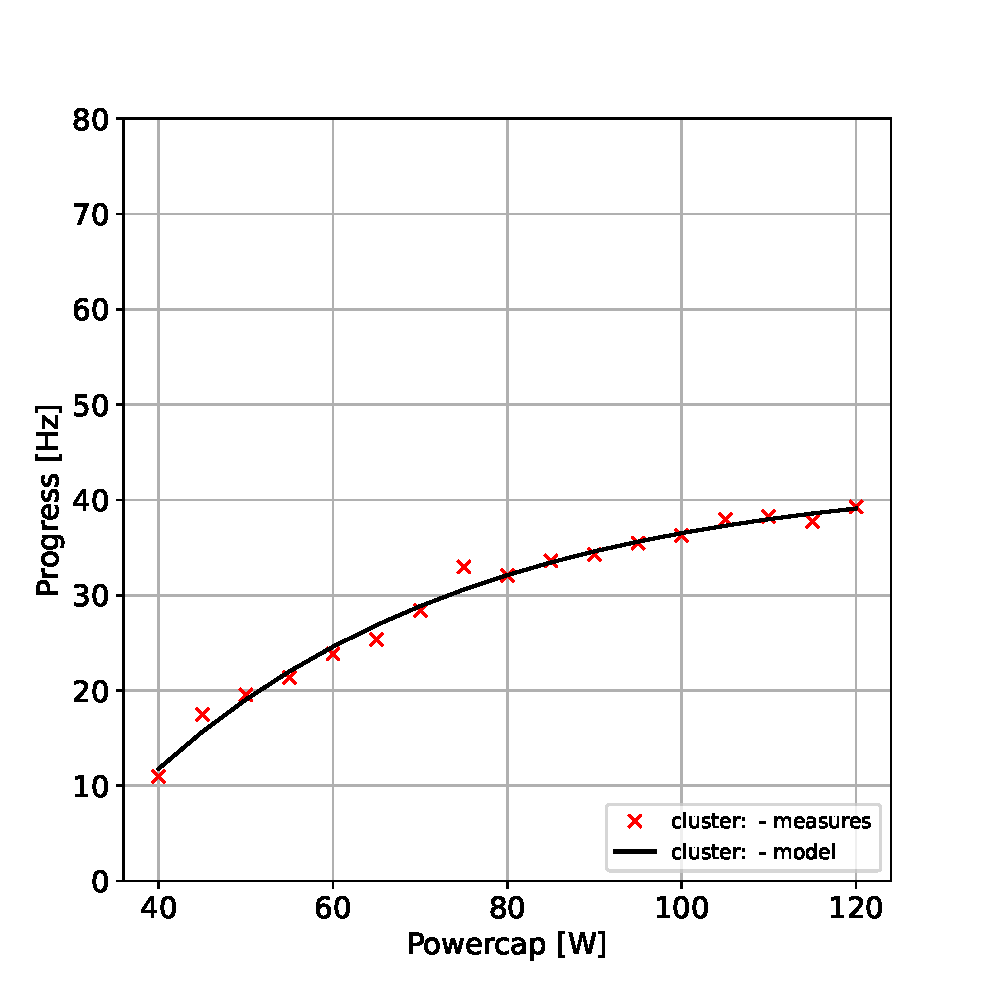
\includegraphics[trim={0cm 0cm 0cm 1.8cm},clip,width = \linewidth]{Figures/non-linear.pdf}
%     \vspace{-0.8cm}
%     \caption{Mathematical model of an HPC node representing the non-linear relation existing between PCAP and progress, obtained using static characterization, showing the data points (red '$\times$') and the best fit curve (black '$-$'). }
%     \label{fig:non-linear}
% \end{figure}
% % \vspace{-1cm}
% \begin{figure}[htb]
% \vspace{-0.5cm}
%     \centering
%     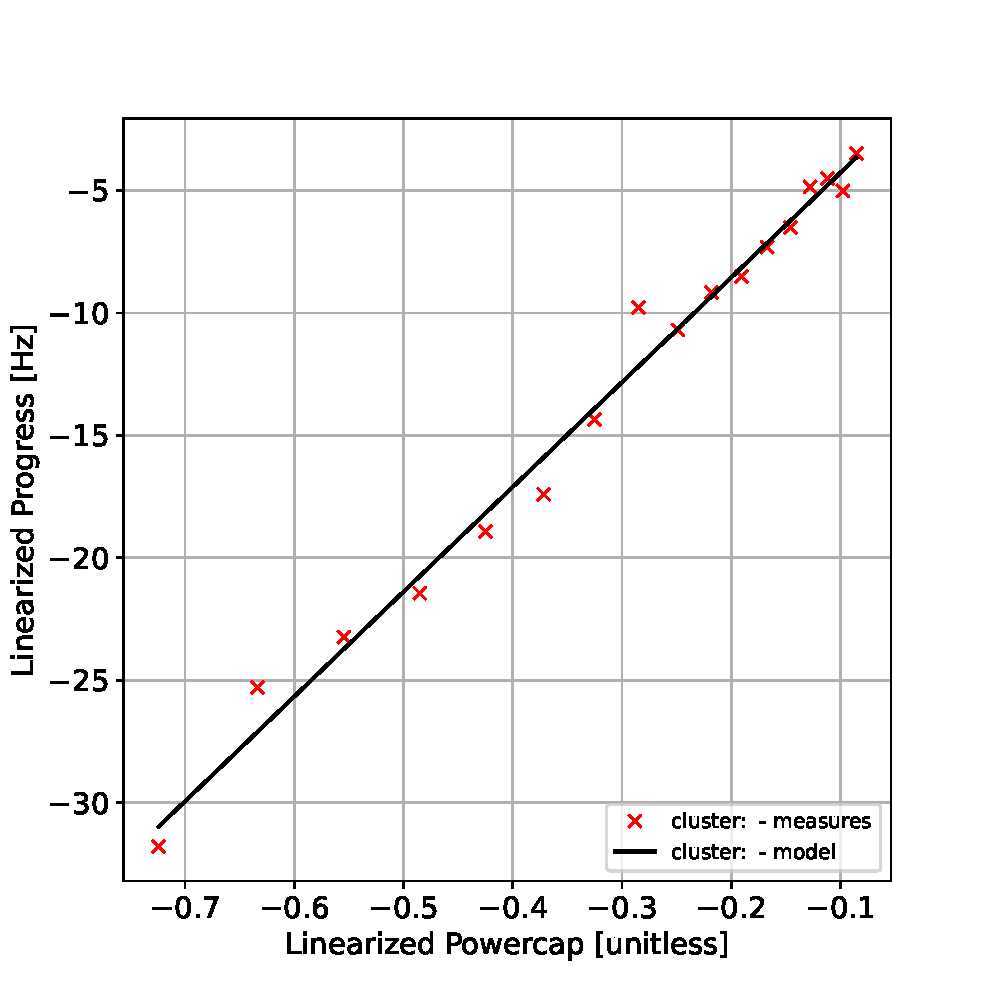
\includegraphics[trim={0cm 0cm 0cm 1.8cm},clip,width = \linewidth]{Figures/linear.pdf}
%     \vspace{-0.8cm}
%     \caption{Linearized model of an HPC node with the axes depicting the region of operation.}
%     \label{fig:linear}
% \end{figure}


% \begin{figure*}[htbp]
%     \centering
%     \subfigure[Mathematical model of an HPC node representing the non-linear relation existing between PCAP and progress, obtained using static characterization, showing the data points (red '$\times$') and the best fit curve (black '$-$'). ]{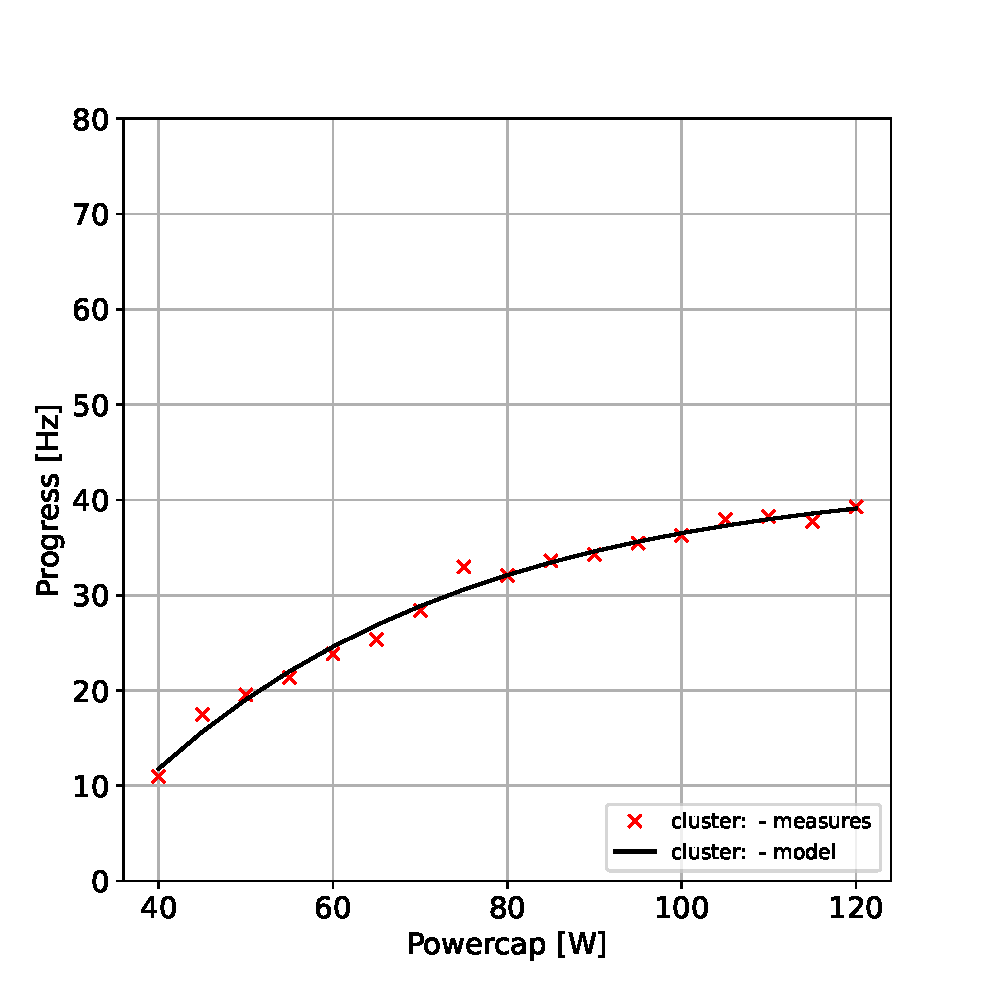
\includegraphics[trim={0cm 0cm 0cm 1.8cm},clip,width = 0.45\linewidth]{Figures/non-linear.pdf}}
%     % \label{fig:non-linear}
%     \hfil
%     \subfigure[Linearized model of an HPC node with the axes depicting the region of operation.]{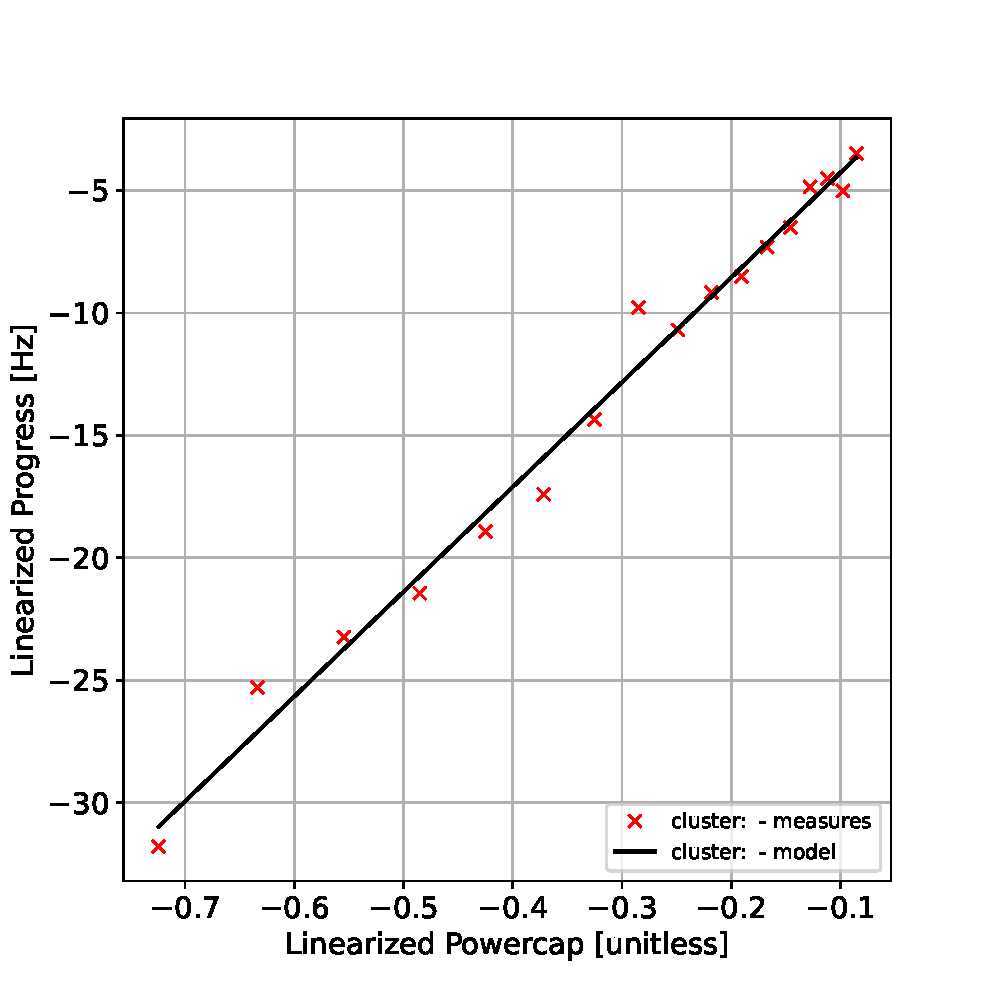
\includegraphics[trim={0cm 0cm 0cm 1.8cm},clip,width = 0.45\linewidth]{Figures/linear.pdf}}
%     % \label{fig:linear}
%     % \caption{}
% \end{figure*}


\begin{figure}[htb]
    \centering
    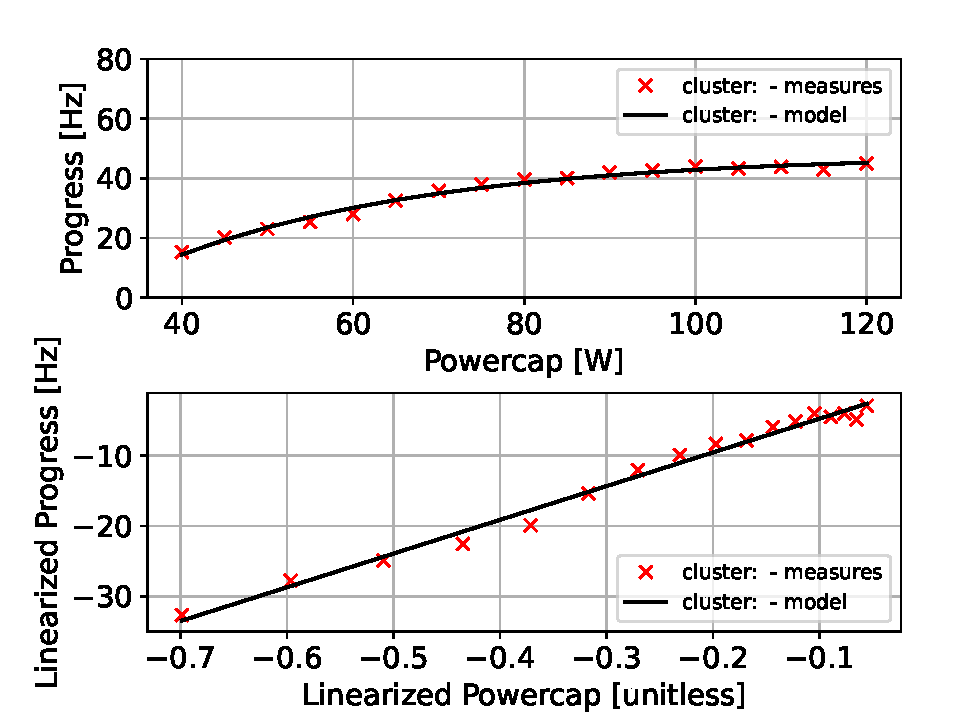
\includegraphics[trim={0.5cm 0.1cm 0cm 0.5cm},clip,width = \linewidth]{Figures/4ab.pdf}
    \vspace{-0.5cm}
    \caption{Mathematical model of an HPC node representing the non-linear and the corresponding linear relations existing between PCAP and progress, obtained using static characterization, showing the data points (red '$\times$') and the best fit curve (black '$-$').}
    \label{fig:static_characterization}
\end{figure}


\begin{table}[htb]
\setlength{\tabcolsep}{1em}
\begin{center}
\begin{tabular}{*{5}{l}}
	\toprule
	Description & Notation & Unit & Value \\
	\midrule
	RAPL slope & {$a$} & [1] & 0.95 \\
	RAPL offset & {$b$} & [W] & 0.15 \\
	            & {$\alpha$} & [W\textsuperscript{-1}] & 0.041\\
	power offset & {$\beta$} & [W] & 24.3  \\
	linear gain & {$K_L$} & [Hz] & 47.9  \\
	time constant & {$\tau$} & [s] & 1/3 \\
	\bottomrule
\end{tabular}
\end{center}
\caption{Model parameters obtained using static characterization of an Intel Xeon Gold 6126 processor.}
\label{tab:static-coefficients}
\vspace{-0.5cm}
\end{table}


% Figures \ref{fig:non-linear} and \ref{fig:linear} shows the results of static characterization.
% Figure \ref{fig:non-linear} shows the nonlinear relation between the performance and power as given by equation \eqref{non_linear_equivalent} and \ref{fig:linear} depicts the relation in \eqref{fig:linear}.  

In the next part  of the experiment, the obtained parameters were used in the mathematical model shown in Equation~\ref{non_linear_equivalent} for generating the next state (progress) in response to an action (PCAP). We employed a PPO-RL agent, to generate a policy and execute it on the mathematical model thereby generating the next state followed by the corresponding reward given by Equation~\ref{ch3:eq:reward_function}. At this point, we would like to bring to the reader's attention that we are not running the application nor the NRM daemon while using the mathematical model. We can implement this training algorithm on any standard processor and do not require any specific hardware. Therefore a simple Python code deploying the PPO-RL agent evaluated the policy, followed by periodic updates which assured its convergence to an optimal value. 

%At this point we would like to hint on the method we discussed before, for determining the choice of reward and the subsequent steps. 
For determining the best reward function that could generate an optimal policy, we performed the training using different reward functions, obtained by varying the $c_1$ and $c_2$ in the Equation~\ref{ch3:eq:reward_function}. We then collected all the models and tested it on the mathematical model to determine its impact on the theoretical performance and power, and determined the region of interest. We also tested these models on the hardware running the application and daemon to compare it against the PI controller.
% We generated this pareto of points as shown in the Figure \ref{fig:execution_time_vs_power} and opted for the reward functions that generated the optimal performance given by the region marked in the blue circle in Figure \ref{fig:execution_time_vs_power}. 

Having determined the optimal reward function, we used the optimal model on the hardware for testing followed by evaluation.
For the testing and evaluation, we reintroduced the hardware and the workload to execute, with the help of NRM. This time, the trained RL-agent provided the PCAP for controlling the power knob of the RAPL actuators. Following this, the corresponding progress values were measured  and fed back into to the RL network to compute the next PCAP. This cycle is repeated till the entire work load is finished execution. 
We repeated the experiment for a variety of scenarios described in the Subsection\ref{subsec:evaluation_steps}.

% The codes relating to the project are made available in the repository attached with the supplementary materials. The static characterization codes are available in the folder titled static characterization.
% After the progress values have settled, we collect all the PCAPs and the corresponding progresses as the data sets which needs the line fitting. Followingly we used the SCIPY regression toolbox to generate the coeffients of an exponential function that best minimized the mean square error (MSE) value. 

% Now using the generated mathematical model which is non-linear in nature we do the linearization to convert it into a markov model as given by the equation \ref{eq:linear_mathematical_model}.
% model is then used for training. For training we. define the RL agent using the stable baselines 3 and test it across 1500  iterations or until the error converges.

% {\color{red}
% \begin{algorithm}
% \caption{Training steps for a PPO-RL agent}
% \begin{algorithmic}
% \State \textbf{Input:} Workload specifications: STREAM benchmark with a total number of iterations: $N$ and total number time-steps in each iterations $n$.
% \State Activate the NRM  and the communication sockets.
% \State Get the information of sensors and  actuators.
% \State Collect the progress sensor values.
% \State Calculate the progress using the median of received heartbeats.
% \State Generate an action PCAP.
% \State Calculate the next state of performance using \ref{mathematical_model}.
% \State Using the next state and the current action calculate the reward using the reward function \ref{reward_function}.
% \State Train the PPO agent using the train. function.
% \end{algorithmic}
% \label{algo:training}
% \end{algorithm}
% }

% \vspace{-1cm}
% The generated model was then tested on a hardware. During the testing phase the processes starting from the workload execution and getting the progress (observation) values followed by generation of an action (policy) are the same. In the next step, instead of testing the policy on a mathematical model we are giving it to the hardware (RAPL actuators) directly instead of the mathematical model. This action, which is optimal, provided the training was successful will make the processor run at that performance just enough to compute the current work load. Thanks to the mathematical modeling (static characterization), the performance was observed to be controlled based on the workload demand. Throughout the paper, the workload is considered static and we expect a constant PCAP (which is optimal) once the execution reaches a stable state. Through this work, we are putting forward a new methodology to regulate the power of a processor while executing a work load. More feature analyzing the characteristics of a work load will be studied in the future experiments.



\subsection{Empirical Results and Discussion} 
\label{Sec:Results}
In this section we will explain the results obtained after following the experiment design described in the previous section. We will also perform the evaluation of the algorithm followed by the interpretation of the results obtained.
% As mentioned before the experiments were performed on the Chameleon Cloud platform. A python code was deployed to synchronize the execution of daemon, workload and the RL-agent. We show here some plots that best explains the experiments and simulation we explained in the previous section.
  
Firstly for choosing an appropriate reward function we trained the RL-agent using the reward function given by the equation \eqref{ch3:eq:reward_function} with varying values of $c_1$ and $c_2$ followed by testing on the mathematical model for its performance.
 The theoretical values of performance (execution time) and the total energy consumed during the execution, were obtained using the control generated by each of the agents and are as shown in the Figure \ref{fig:execution_time_vs_power}.
 % Using this figure we also showed, how we chose appropriate values for the constants $c_1$ and $c_2$ as given in the equation \eqref{ch3:eq:reward_function}. 
 By using a series of values for $c_1$ and $c_2$ starting from 0 followed by increments of 0.1, till 10, we were able to observe the variations in the performance and power for each of the designed reward. As expected we obtained a combination of values for $c_1$ and $c_2$ that yielded respective results ranging from the fastest to the slowest performance as shown in the figures \ref{fig:execution_time_vs_power}.
% The trained model is then tested on the mathematical model to see the varying trends in the execution time and the consumed power.
% Figure \ref{fig:execution_time_vs_power} shows the in real-time, the corresponding power and performance variation during the execution is obtained and is as shown in figure \ref{fig:power_performance_vs_time}.
Observing the figure we can see that there is a point in the maximum curvature region (marked in blue circle) in figure \ref{fig:execution_time_vs_power} that can be considered as an ideal region to look for a candidate reward function. This point corresponds to the minimum energy consumption and the maximum performance. Note that, there were a couple of ideal candidates for the reward function that repeated across multiple execution of this experiment, for example, ($c_1$=1.052,$c_2$=2.22) and ($c_1$=0,$c_2$=4.44) gave the same responses. We chose the model, that was obtained after training using the reward function, $R(t) = -1.052 PCAP(t) + 2.22 \frac{progress(t)}{measured \ power(t)}$, as the RL-agent to control the HPC nodes during the testing phase.
\def\sca{1}
\def\scb{1}
\begin{figure}[htb]
% \vspace{-0.25cm}
  \centering
  \begin{tikzpicture}[remember picture]
    \node[inner sep=0pt,anchor=south west] (A1) {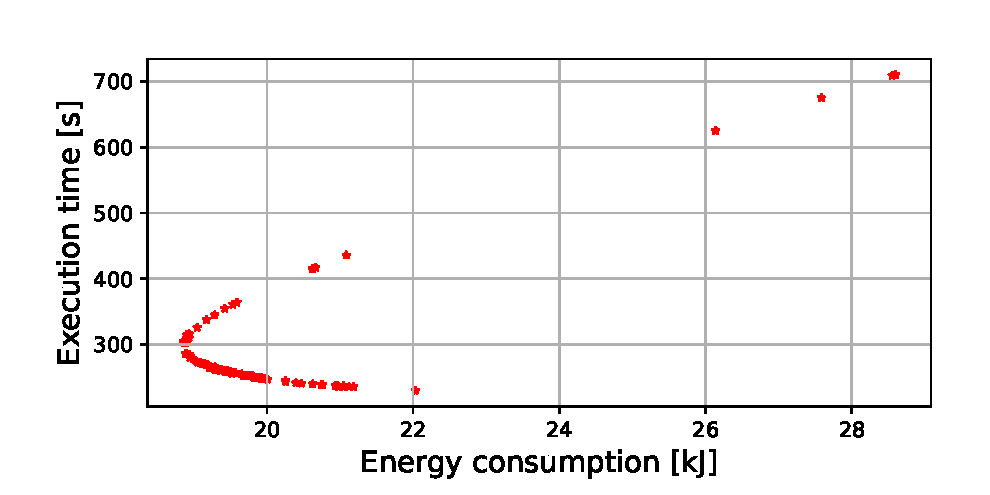
\includegraphics[trim={0.9cm 0cm 1cm 1cm},clip,width=\sca\linewidth]{Figures/pareto_theoretical.pdf}};
    \draw[line width=0.4mm,blue] (\sca*2.6,\sca*2.3) circle (10pt) node[anchor=west]{};
  \end{tikzpicture}
  %% Overlay part
  \begin{tikzpicture}[remember picture,overlay]
  \end{tikzpicture}
  \vspace{-0.75cm}
  \caption{A Pareto of execution time vs energy consumed, generated by varying the RL-agents trained with different reward functions. The x-axis shows the total energy consumed during the execution, and the time of execution is plotted on the y-axis. The ideal characteristics are inside the blue circle.}
  \label{fig:execution_time_vs_power}
\end{figure}
% \vspace{-0.5cm}
% \begin{figure}[htb]
% \vspace{-0.6cm}
%   \centering
%   \begin{tikzpicture}[remember picture]
%     \node[inner sep=0pt,anchor=south west] (A2) {\includegraphics[trim={0cm 0cm 0cm 0cm},clip,width=\scb\linewidth]{Figures/result_all_2022-11-01 06:25:49.650753.png}};
%     \draw[line width=0.4mm,blue] (\scb*5,\scb*6.12) circle (18pt) node[anchor=west]{};
%     \draw[line width=0.4mm,blue] (\scb*5,\scb*2) circle (18pt) node[anchor=west]{};
%   \end{tikzpicture}
%   %% Overlay part
%   \begin{tikzpicture}[remember picture,overlay]
%   \end{tikzpicture}
%   \vspace{-0.6cm}
%   \caption{Plot of power and progress vs time steps. The x-axis of both the figures represents the time steps during the execution while the y-axis represents the corresponding progress and action values respectively. The blue circle depicts the optimal working condition identified in the figure \ref{fig:execution_time_vs_power}.}
%   \label{fig:power_performance_vs_time}
% \end{figure}
% In the next part of this section we will explain the evaluation of the obtained results in detail.
% \begin{figure}
% \begin{tikzpicture}[]
%     \node[inner sep=0pt,anchor=south west](A1){\includegraphics[width=0.4\linewidth]{Figures/result_2022-10-19 15:24:56.044367.pdf};
%     \draw[black] (-3,-1.5) circle (20pt) node[anchor=west]{};
%     \includegraphics[width=0.4\linewidth]{Figures/result_2022-10-19 16:14:27.993949.png};
%     \draw[black] (-3,-1.5) circle (20pt) node[anchor=west]{};
%     \label{fig:find_optimal}
% \end{tikzpicture}
% \caption{test}
% \end{figure}

% \begin{figure}
%     \centering
%     \includegraphics[height = 8cm, width = 9cm]{Figures/result_2022-10-19 15:24:56.044367.pdf}
%     \caption{Generating performance indices using various reward functions (RL method)}
%     \label{fig:choose_reward_1}
% \end{figure}
    
% \begin{figure}
%     \centering
%     \includegraphics[height = 7cm, width = 9cm]{Figures/result_2022-10-19 16:14:27.993949.png}
%     \caption{Performance and Power for varying reward functions (RL method)}
%     \label{fig:choose_reward_2}
% \end{figure}



\subsection{Analysis of Results}\label{subsec:Evaluation}
Before we proceeded with the analysis and evaluation of the proposed optimal controller for the PCAP, we needed to verify its performance by comparing it against the existing PI controller. For that, we needed to run both the algorithms on the same machine. We first executed the PI controller on the HPC node with varying set-points as shown in the Figure ~\ref{fig:comparison_PI_RL_controller}. The pareto of points with gradients of colors ranging from yellow to blue depicts the result obtained for the PI controller with varying setpoints. The setpoint was specified using the parameter $\epsilon$, representing the allowed tolerance in the maximum performance value. The $\epsilon$ value was varied from 0 to 0.6 randomly, during the experiments using PI controller. The shortest execution time of 240\unit{\second} (corresponding to faster execution) was obtained at an energy consumption of 36\unit{\kilo \joule} at an $\epsilon$ value of 0.1.
The setpoint value is expected to change based on the hardware being tested, whose dependency on the controller is being removed while using an RL controller. 
We then tested the trained RL controllers on the same hardware running the application and created a similar pareto of points. In the Figure ~\ref{fig:comparison_PI_RL_controller}, the red points represent the response of the HPC node controlled using the trained RL-agent. We observed that the optimal region consisted of points vary close to the best performance obtained using the PI controller. It was observed that the $R(t)$ proposed in the previous subsection fell within a closer range of the best performance.
\begin{figure}[htb]
    \centering
    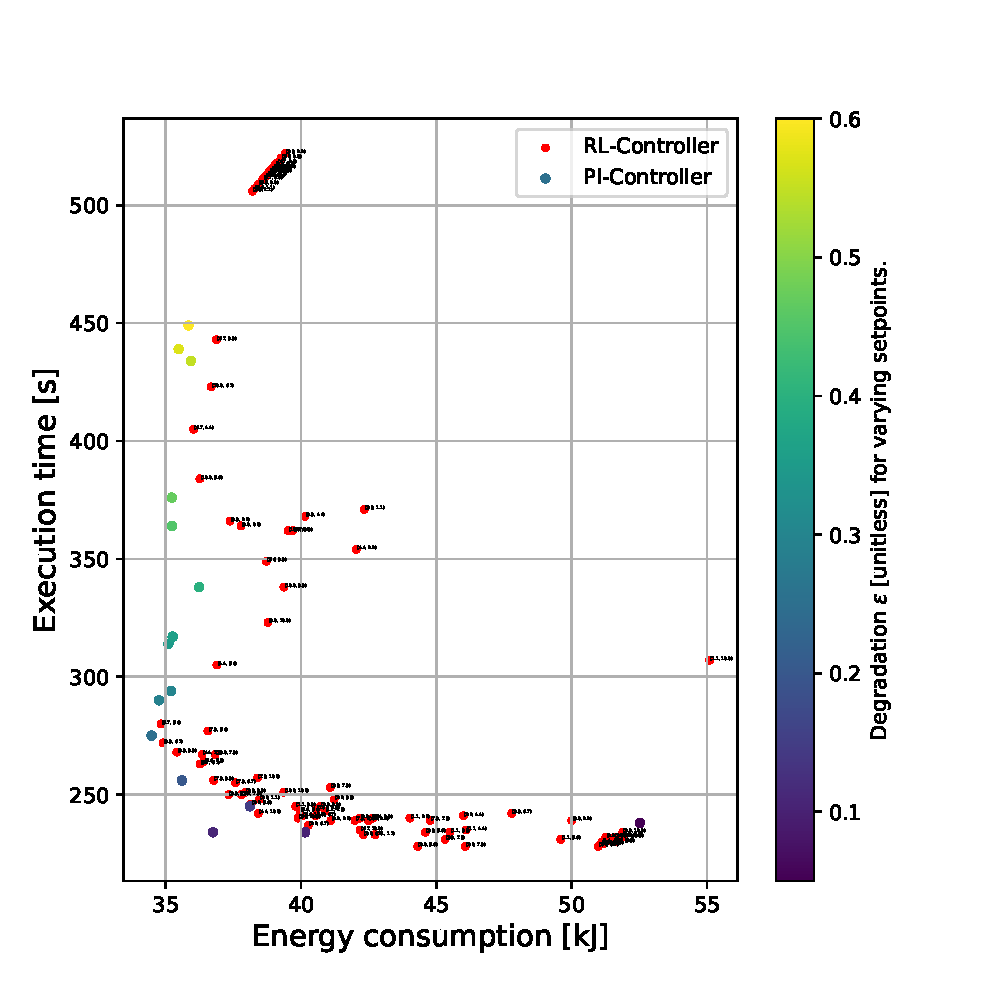
\includegraphics[trim={0.5cm 0.4cm 1.5cm 1.9cm},clip,width = \linewidth]{Figures/pareto_real.pdf}
    \vspace{-0.5cm}
    \caption{Plot showing the comparison of PI controller with varying setpoints (values for $1- \epsilon$) and RL controller for varying reward functions. The PI control objective is given as a degradation factor $\epsilon$, that is, the tolerable loss of performance}
    \label{fig:comparison_PI_RL_controller}
    % \vspace{-0.5cm}
\end{figure}

Through these comparisons we were able to justify the use of a trained RL-agent as an optimal controller aimed to minimize the power consumption. Using the proposed RL controller, we were able to regulate the HPC node performance around those regions of operation, where a PI controller was regulating the performance, given a user-defined set-point. We also were able to excite the HPC node at some other regions where a slower response was obtained but at a very low energy consumption. We will now look for points where optimal performance and power consumption was recorded and will check for the repeatability of the experiments using the same hardware as well as different hardware.

We used the RL-agent trained using the reward function chosen previously, for the remaining part of the experiment consisting of:
\begin{itemize}
% \item Comparison with the PI controller
\item Repeatability on the same node and
\item Repeatability on different nodes.
\end{itemize}

Within each of these analysis, we considered two different scenarios to compare with the performance of the proposed method, namely:
% The experiments were performed to simulate three different scenarios with:
\begin{itemize}
\item Maximum PCAP: allowing the node to utilize the maximum allowed capabilities of the system,
% \item Optimal PCAP: control using the proposed method,
\item Minimum PCAP: limiting the performance, by allowing only the minimum power at the actuators.
\end{itemize}

% Figures \ref{fig:comparison_execution_time} and \ref{fig:comparison_power} compares the power and execution time associated with the three experimental scenarios:
% The implementation code for the PI controller was taken from the paper \cite{cerf2021sustaining} artifacts and was deployed on an Intel(R) Xeon(R) Gold 6126 CPU @ 2.60GHz. The implementation used the same mathematical model that was generated using the static characterization and the experiment was performed for 13 different set points ranging from the minimum and maximum allowed performance measures. We then used the proposed RL controller trained using different reward functions. A variety of around 100 reward functions were considered to excite the hardware at various zones of its allowed performance. The results are as shown in the Figure \ref{fig:comparison_PI_RL_controller}.



For the analysis of the repeatability of the experiment on the same node, we conducted a total of 30 executions of the experiment with RL controller being used for 10 of the executions. In the remaining 20 executions we used the maximum allowed and minimum allowed values for the PCAP to record the statistics. We didn't consider the PI controller for the comparison here, since we are only evaluating the repeatability of the proposed method. We then observed the statistics associated with each set of executions and the values are tabulated.  
% Figures \ref{fig:comparison_execution_time} and \ref{fig:comparison_power} shows the obtained results.
Figure \ref{fig:comparison_execution_time} depicts the results of the experiment with the execution time plotted against the energy consumed during the each of the experiments. Figure \ref{fig:comparison_power} shows the values of instantaneous PCAPs sensed during each time step, by the RAPL sensors for three different executions using maximum, minimum and optimal PCAP respectively. 
% related statistics obtained are as shown in the table. \ref{tab:statistics_repeatability}:
% \begin{table}[htb]
% \setlength{\tabcolsep}{1em}
% \begin{center}
% \begin{tabular}{*{5}{l}}
% 	\toprule
% 	Control & Mean ET[\unit{\second}] & Std.Dev ET & Mean EC[\unit{\kilo\joule}] & Std.Dev EC\\
% 	\midrule
% 	Optimal & 315.75 & 5.89 & 43.99 & 0.744\\
% 	Minimal & 555.78 & 26.20 & 41.97 & 5.9 \\
% 	Maximal & 242.75 & 3.6 & 60.50 & 0.77  \\
% 	\bottomrule
% \end{tabular}
% \end{center}
% \caption{Statistics in repeatability}
% \label{tab:statistics_repeatability}
% \end{table}
% Comparing the results are as shown in figure \ref{fig:comparison_execution_time} and \ref{fig:comparison_power}
% \vspace{-0.3cm}
\begin{figure}[htb]
    \centering
    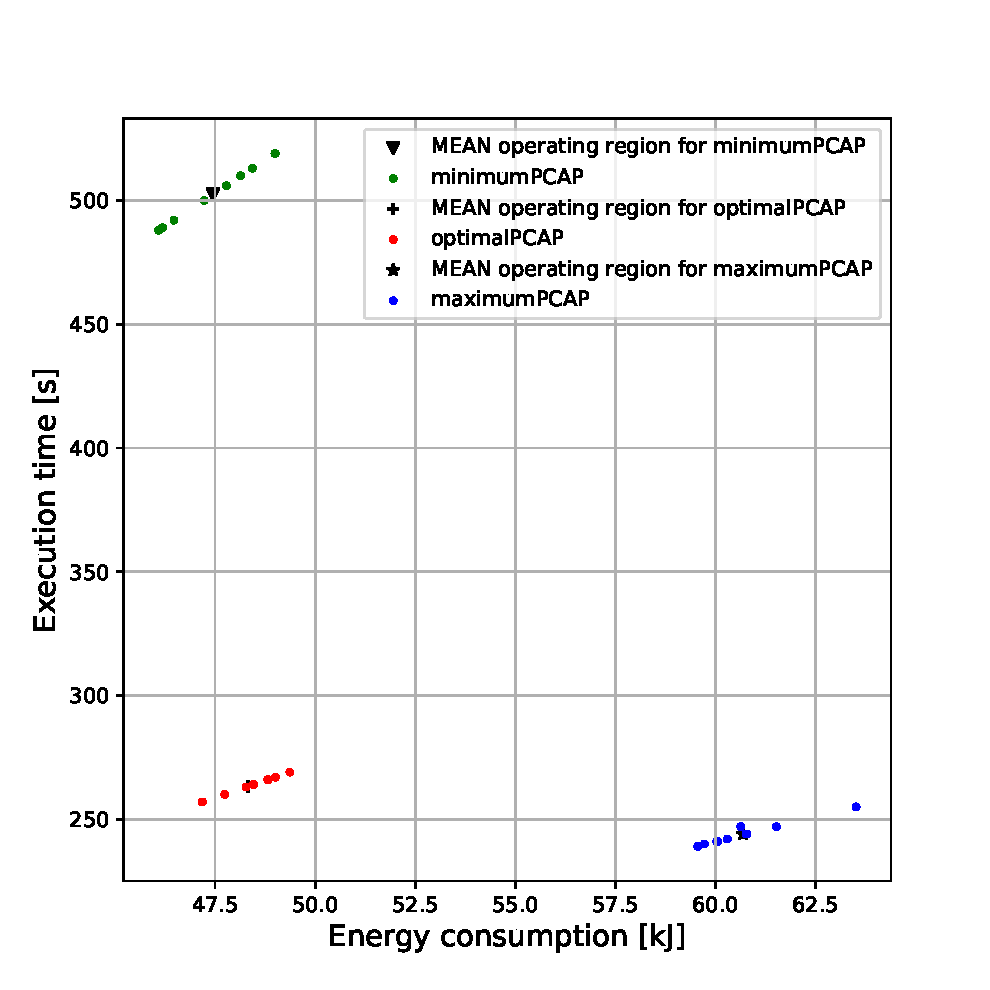
\includegraphics[trim={0.5cm 0.5cm 0.5cm 2cm},clip,width=\linewidth]{Figures/repeatability.pdf}
    % \vspace{-0.9cm}
    \caption{Comparison of the execution-time and the energy consumed during the execution of the experiments performed on the same hardware employing three different methods. The statistics of the executions are shown in the table \ref{tab:statistics_repeatability}}
    \label{fig:comparison_execution_time}
\end{figure}
\begin{figure}[htb]
    \centering
    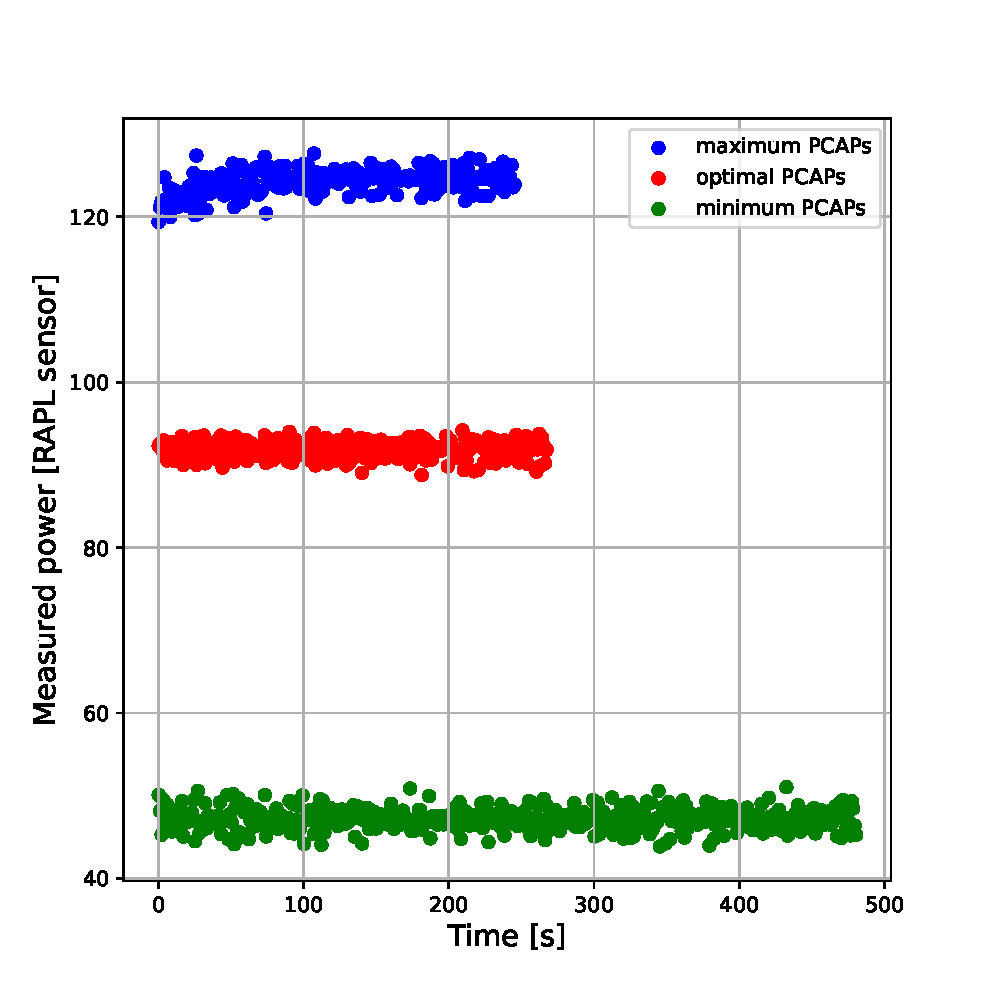
\includegraphics[trim={0.5cm 0.5cm 0.5cm 2cm},clip,width=\linewidth]{Figures/time_stamps.pdf}
    % \vspace{-0.9cm}
    \caption{Instantaneous power vs time-steps plots for a single execution of the experiment using optimal, maximum and minimum PCAP controllers.}
    \label{fig:comparison_power}
\end{figure}
{
In Figure \ref{fig:comparison_execution_time}, ensuring the maximum PCAP for the RAPL actuators, that put no limit on the amount of energy drawn into the system, the workload execution was completed in 245\unit{\second}. But when we look at the total energy consumed over the period it was in the range of an average value of 60.97\unit{\kilo\joule}. On the other hand, enforcing the minimum PCAP on RAPL actuators, the power consumption was minimal, i.e in the range of an average value of 47.49\unit{\kilo\joule} of energy, but compromising on the total execution time which lasted for 501.14\unit{\second}. On the other hand, the RL based controller was able to limit the power consumption and comparable execution time. It was observed that the average power consumption, over 10 experiments using the optimal PCAP, was 48.23\unit{\kilo\joule}, while the average execution time was 261.19\unit{\second}. This shows a reduction of 21\% on the consumed power, while the performance was compromised only by 6.5\%.} The statistics of the experiment are given in the table \ref{tab:statistics_repeatability}
\begin{table}[htb]
\setlength{\tabcolsep}{1em}
\begin{center}
\begin{tabular}{*{5}{l}}
	\toprule
	{} & Minimal & Maximal & Optimal \\
	\midrule
	$\mu$ Execution Time [\unit{\second}] & 501.14 & 245.23 & 261.19.\\
    $\sigma$ Execution Time & 26.20 & 3.6 & 5.89 \\
    $\mu$ Energy Consumption [\unit{\kilo \joule}] & 47.49 & 60.97 & 48.23 \\
    $\sigma$ Energy Consumption & 1.98 & 0.77 & 0.744 \\
	\bottomrule
\end{tabular}
\end{center}
\caption{Statistics of repeatability using the same node over 10 executions. $\mu$ and $\sigma$ depict mean and standard deviation respectively.}
\label{tab:statistics_repeatability}
\vspace{-0.5cm}
\end{table}
% \todo{this is a very good idea, but I hope each experiment was repeated on each hardware}

For the next part, we performed a total of 21 exections consisting of 7 sets with 3 executions each with maximum, minimum and optimal PCAP. Each set was exectuted on different hardware. We made the reservation for 7 nodes from the Chameleon Cloud using a single lease in-order to assure diversity in hardware. The results of the execution was then gathered for analysis of its statistics. 
\begin{figure}[htb]
    \centering
    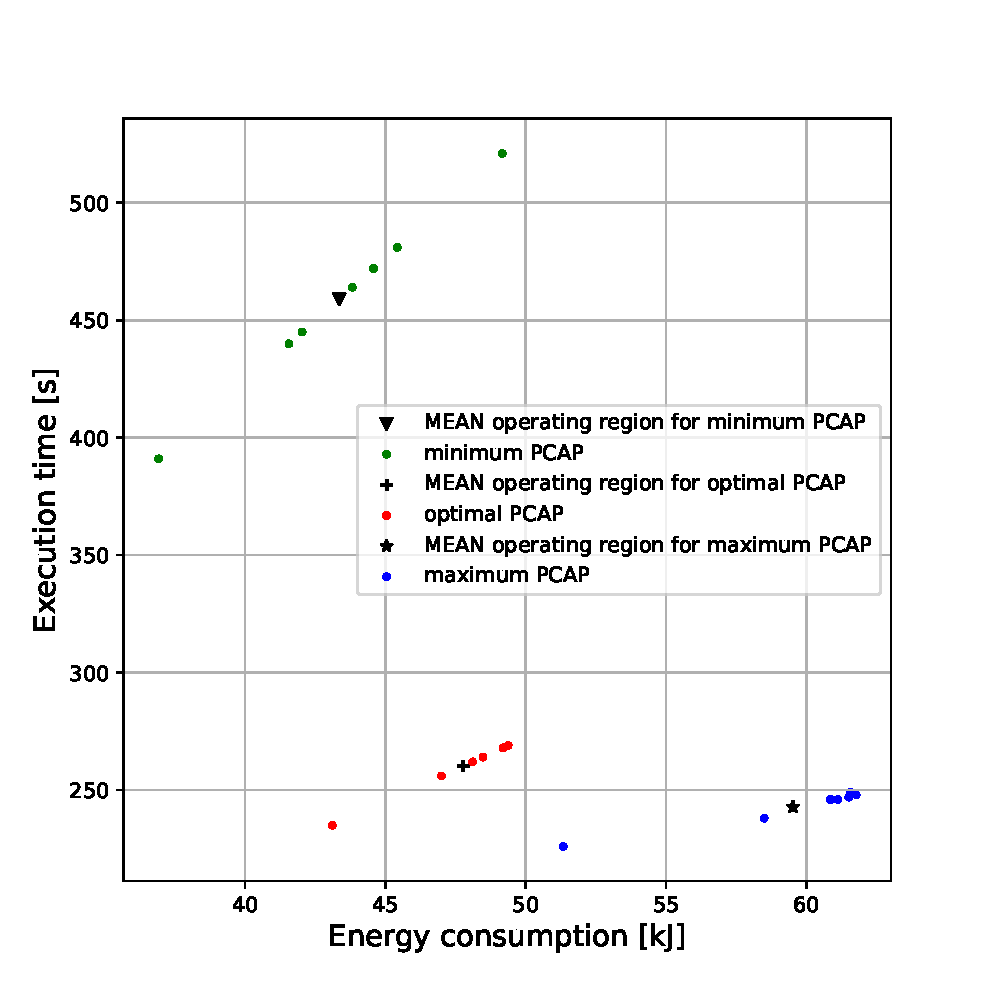
\includegraphics[trim={0.5cm 0.5cm 0.5cm 2cm},clip,width=\linewidth]{Figures/viability.pdf}
    % \vspace{-0.75cm}
    \caption{Comparison of the execution-time and the energy consumed during the execution of experiments, performed on different nodes using the three methods. The statistics of the executions are shown in the table \ref{tab:statistics_repeatability_diff_nodes}}
    \label{fig:comparison_execution_time_diff_nodes}
\end{figure}
Figure \ref{fig:comparison_execution_time_diff_nodes} shows the obtained results of the experiment. It was observed that the proposed RL based controller was able to bring down the energy consumption by 19.7\% at a cost of 7.3\% in performance.
It was also observed that the variance among each set of the experiments have gone high due to the changes in hardware, but in effect the optimal controller performed with the minimum variance. The related statistics are presented in the table \ref{tab:statistics_repeatability_diff_nodes}.
\begin{table}[htb]
\setlength{\tabcolsep}{1em}
\begin{center}
\begin{tabular}{*{5}{l}}
	\toprule
	{} & Minimal & Maximal & Optimal \\
	\midrule
	$\mu$ Execution Time [\unit{\second}] & 459.14 & 242.85 & 260.28\\
    $\sigma$ Execution Time  & 40.21 & 8.25 & 12.03 \\
    $\mu$ Energy Consumption [\unit{\kilo \joule}] & 43.3 & 59.52 & 47.78 \\
    $\sigma$ Energy Consumption & 3.78 & 3.77 & 2.22 \\
	\bottomrule
\end{tabular}
\end{center}
\caption{Statistics of repeatability over 5 executions on different HPC nodes. $\mu$ and $\sigma$ have the usual meaning.}
\label{tab:statistics_repeatability_diff_nodes}
\end{table}
Through the repeatability experiments we were able to prove the reliability of the proposed approach for generating an optimal control for HPC nodes. We were also able to verify that the energy consumption reduction is consistent throughout its execution irrespective of the hardware.

\section{Conclusion}\label{ch3:sec:Conclusion}
This paper addresses the problem of managing power consumption in heterogeneous data center compute nodes by focusing on the potential of dynamically adjusting power across
compute elements to save energy with almost no impact on performance.
Our approach involves model-based reinforcement learning that learns using a mathematical model, which is generated using static characterization of a specific hardware node running a standard application benchmark. The control of the hardware, then uses the trained RL agent to ensure optimal performance. Experimental validation shows promising results for systems running a memory-bound benchmark. The repeatability of results showed a standard deviation of 5.89 with a mean energy consumption of 48.23 \unit{\kilo \joule} during 261.19\unit{\second} of mean execution time. These results indicate that the RL-based approach can serve as an alternative to the PI controllers used in our past experiments in order to remove the dependency on operational setpoints. The approach presented in this paper is most suitable for cloud providers and high performance compute node administrators who seek solutions to reduce power consumption of their server resources yet not impact application performance. In our future work, we aim to resolve the dependency of the proposed work on the mathematical model for training. We also seek to design a generalized RL-based controller, controlling PCAPs on nodes executing a variety of applications.
% Akhilesh, is there a guthub url?
% \todo{identify the limits, be explicit, we don't ponder in papers}

\section*{Acknowledgments}\label{sec:Acknowledgments}
Results presented in this paper were obtained using the Chameleon testbed supported by the National Science Foundation.
Argonne National Laboratory's work was supported by the U.S. Department of Energy, Office of Science, Advanced Scientific Computer Research, under Contract DE-AC02-06CH11357. This research was supported by the Exascale Computing Project (17-SC-20-SC), a collaborative effort of the U.S. Department of Energy Office of Science and the National Nuclear Security Administration. The dataset and the codes used for the entire experiment, including the static characterization, training and testing, are hosted on our  \href{https://github.com/akhileshraj91/GENERALIZED_RL_ANL.git}{GitHub repository}. 
% We also provide with the readers, a complete access to our \href{https://chi.tacc.chameleoncloud.org/ngdetails/OS::Glance::Image/9c96d38c-61ab-4b55-bec1-bd115f05c06a}{Chameleon Cloud image} that will help them recreate the results. 
We also provide readers with complete access to our \href{https://chi.tacc.chameleoncloud.org/ngdetails/OS::Glance::Image/f6974b54-93fc-4140-9163-7aae9fc3070d}{Chameleon Cloud image}, which will enable them to reproduce the results.

% \todo{public ref? snapshot of the chameleon setup?}
% \clearpage

